\documentclass[13pt,a4paper]{report}
\usepackage[margin=0.6in]{geometry}
\usepackage{fancybox}
\usepackage[utf8]{inputenc}
\usepackage[vietnamese,main=english]{babel}
\usepackage{multicol}
\usepackage{tabularx}
\usepackage{lmodern}
\usepackage{minted}
\usepackage{indentfirst}
\usepackage{float}
\usepackage{enumitem}
\usepackage{afterpage}
\usepackage[super]{nth}
\usepackage{titlesec}
\usepackage{bigdelim}
\usepackage[titles]{tocloft}
\usepackage{makecell}
\usepackage{arydshln}
\usepackage{perpage} %the perpage package
\usepackage{graphicx}
\usepackage{caption}
\usepackage{gensymb}
\usepackage{tikz}
\usepackage{circuitikz}
\usepackage{pgfplots}
\usepackage{cancel}
\usepackage{xurl}
\usepackage[bottom]{footmisc}
\usepackage[font=footnotesize,labelfont={scriptsize}]{subfig}
\usepackage{wrapfig}
\usepackage{latexsym,amssymb,amsmath}
%\usepackage{algpseudocode}
\usepackage{tocvsec2}
\usepackage{fancyref}
\usepackage{bookmark}
\usepackage{hyperref}
\usepackage[nameinlink,noabbrev]{cleveref}

\newcolumntype{Y}{>{\centering\arraybackslash}X}

\PassOptionsToPackage{hyphens}{url}

\makeatletter
\pgfcircdeclarebipole{}{\ctikzvalof{bipoles/vsourceam/height}}{vsourceAM}{\ctikzvalof{bipoles/vsourceam/height}}{\ctikzvalof{bipoles/vsourceam/width}}{%
  \pgfsetlinewidth{\pgfkeysvalueof{/tikz/circuitikz/bipoles/thickness}\pgfstartlinewidth}
   \pgfpathellipse{\pgfpointorigin}{\pgfpoint{0}{\pgf@circ@res@up}}{\pgfpoint{\pgf@circ@res@left}{0}}
   \pgfusepath{draw}
   \pgfscope
       \pgftransformxshift{0.6*\ctikzvalof{bipoles/vsourceam/margin}\pgf@circ@res@left}
       \pgftext[rotate=-\pgf@circ@direction]{$+$}
       \pgfusepath{draw}
   \endpgfscope
   \pgfscope
       \pgftransformxshift{0.6*\ctikzvalof{bipoles/vsourceam/margin}\pgf@circ@res@right}
       \pgftext[rotate=-\pgf@circ@direction]{$-$}
       \pgfusepath{draw}
   \endpgfscope
}
\makeatother

\MakePerPage{footnote} %the perpage package command
\usetikzlibrary{shapes,positioning,arrows,calc}

\newcommand*\justify{%
  \fontdimen2\font=0.4em% interword space
  \fontdimen3\font=0.2em% interword stretch
  \fontdimen4\font=0.1em% interword shrink
  \fontdimen7\font=0.1em% extra space
  \hyphenchar\font=`\-% allowing hyphenation
}
\renewcommand\cftchapafterpnum{\vskip-2pt}
\renewcommand\cftsecafterpnum{\vskip-2pt}

\renewcommand{\theequation}{\arabic{equation}}

% FLOW CHART
\tikzstyle{startstop} = [rectangle, rounded corners, minimum width=3cm, minimum height=1cm,text centered, draw=black, fill=red!30]
\tikzstyle{io} = [trapezium, trapezium left angle=70, trapezium right angle=110, minimum width=3cm, minimum height=1cm, text centered, draw=black, fill=blue!30]
\tikzstyle{process} = [rectangle, minimum width=3cm, minimum height=1cm, text centered, draw=black, fill=orange!30, text width=4cm]
\tikzstyle{decision} = [diamond, aspect=2.5, minimum width=3cm, minimum height=1cm, text centered, draw=black, fill=green!30]
\tikzstyle{arrow} = [thick,->,>=stealth]

% CHAPTER FORMAT
\titleformat{\chapter}%[display]
{\bfseries\fontsize{25}{30}\selectfont\raggedright}% Format and size of title text
{\llap{%
    \rule[-6pt]{6cm}{1.18cm}\rule{6pt}{0pt}}% Black box to the left, lowered 6pt. The end rule is a horisontal space.
  \llap{% Number also to the left, on top of the black box.
    \fontsize{30}{44}\selectfont\color{white}\thechapter\rule{10pt}{0pt}}}{0pt}{}{}

\counterwithin{figure}{section}
\renewcommand{\thefigure}{\arabic{chapter}.\arabic{section}.\alph{figure}}

\renewcommand{\thetable}{\arabic{table}}

\renewcommand\labelitemi{$-$}
  
\titleformat{\section}
  {\LARGE\bfseries}{}{}{}
\renewcommand\thesection{\arabic{section}.}
\renewcommand\thesubsection{\arabic{subsection}}
\makeatletter
\renewcommand*\l@section{\@dottedtocline{1}{1.5cm}{2em}}
\renewcommand\section{\@startsection {section}{1}{-1em}%
  {-3.5ex \@plus -1ex \@minus -.2ex}%
  {2.3ex \@plus.2ex}%
  {\normalfont\Large\bfseries}}
\def\sectionmark#1{%
      \markright {\MakeUppercase{#1}}}
\makeatother

\titleformat{\subsection}
  {\normalfont\bfseries}{\thesubsection.}{0.5em}{}
\renewcommand\cftsubsecaftersnum{.} 
\renewcommand\thesubsection{\alph{subsection}}

\addto{\captionsenglish}{%
  \renewcommand{\bibname}{References}
}

%\addtocontents{toc}{\setcounter{tocdepth}{2}}
%\addtocontents{lof}{\vskip -1.6cm}
%\addtocontents{lot}{\vskip -1.6cm}

    
% TOC settings
\renewcommand\cftchapnumwidth{2.8em}
\renewcommand\cftsecnumwidth{3em}
\renewcommand\cftsecindent{3em}
\renewcommand\cftsubsecindent{5em}
\renewcommand\thechapter{\Roman{chapter}}
    
%\titleformat{\chapter}[display]{\normalfont\huge\bfseries}{}{0pt}{\Huge}
\newcommand{\hsp}{\hspace{20pt}}
%\titleformat{\chapter}[hang]{\Huge\bfseries}{\thechapter\hsp\textcolor{gray75}{|}\hsp}{0pt}{\Huge\bfseries}
\titleformat*{\subsubsection}{\large\bfseries}
%\titlespacing*{\chapter}{0pt}{0pt}{0pt}
    
\newcolumntype{P}[1]{>{\centering\arraybackslash}p{#1}}
\newcolumntype{C}{>{\centering\arraybackslash}p{4em}}
    
\setlist[itemize]{noitemsep, topsep=0pt}
%\AtBeginEnvironment{multicols}{\RaggedRight}

\titlespacing*{\chapter}{0pt}{0pt}{20pt}

\newcommand\Chapter[2]{\chapter
  [#1\text{: }\hfil\hbox{}\protect\linebreak{\itshape#2}]%
  {#1\\[-0.75ex]\Large#2}%
  \markboth{\MakeUppercase{\chaptername\ \thechapter.\ #1}}{}%
}


\def\doubleoverline#1{\overline{\overline{#1}}}

\captionsetup[subfloat]{labelformat=empty}

\begin{document}
%Trang bìa 1
\fontsize{13pt}{18pt}\selectfont
\begin{titlepage}
\thispagestyle{empty}
\thisfancypage{%đóng khung trang này
\setlength{\fboxsep}{0pt}% 8pt là độ dày của đường viền
\fbox}{} % phần nội dung sau là tương tự như đã làm
\

\begin{center}
\begin{large}
HO CHI MINH CITY UNIVERSITY OF TECHNOLOGY $-$ VNU HCMC
\end{large} \\
\begin{large}
OFFICE FOR INTERNATIONAL STUDY PROGRAM
\end{large} \\
\begin{large}
FACULTY OF ELECTRICAL AND ELECTRONIC ENGINEERING
\end{large} \\
\textbf{--------------------  *  --------------------}\\[4cm]
\includegraphics[scale=0.1]{logobk.png}\\[1cm]
{\fontsize{20pt}{1}\selectfont DIGITAL SYSTEMS (LAB)}\\
{\fontsize{20pt}{1}\selectfont EXPERIMENTAL REPORT (Lab 2)}\\[2.5cm]
\end{center}

\begin{otherlanguage}{vietnamese}
\begin{tabbing}
	\hspace{3.5cm}Lecturer  \ \ \ \ \=: \textbf{\parbox[t]{9cm}{Mr. Nguyễn Tuấn Hùng}}\\
	\hspace{3.5cm}Subject \>: \textbf{\parbox[t]{12cm}{Digital Systems}}\\
	\hspace{3.5cm}Class \>: \textbf{\parbox[t]{9cm}{TT06}}\\
	\hspace{3.5cm}Name \>: \textbf{\parbox[t]{9cm}{
		Lương Triển Thắng}}\\
	\hspace{3.5cm}Student ID \>: \textbf{\parbox[t]{9cm}{
		2051194}}\\[40pt]
\end{tabbing}
\end{otherlanguage}

\vspace{2.25cm}
\begin{center}
{\fontsize{13pt}{1}\selectfont Ho Chi Minh City, \nth{7} June, 2022}
\end{center}
\end{titlepage}

\tableofcontents

\setminted{fontsize=\normalsize}

\setcounter{chapter}{1}

\Chapter{Laboratory 2}{Adder and flip-flop}

\section{Known how to program 4-bit adder}

\ctikzset{logic ports=ieee}

\subsection{Code}
\subsubsection{FA.vhd}
\begin{minted}{vhdl}
LIBRARY ieee;
USE ieee.std_logic_1164.ALL;

ENTITY Exc1 IS
	PORT (
		a : IN STD_LOGIC;
		b : IN STD_LOGIC;
		ci : IN STD_LOGIC;
		s : OUT STD_LOGIC;
		co : OUT STD_LOGIC
	);
END Exc1;

ARCHITECTURE arch OF Exc1 IS
BEGIN
	s <= a XOR b XOR ci;
	co <= (a AND b) OR (ci AND (a XOR b));
END ARCHITECTURE;
\end{minted}

\subsubsection{Exc1.vhd}
\begin{minted}{vhdl}
LIBRARY ieee;
USE ieee.std_logic_1164.ALL;
USE ieee.numeric_std.ALL;

ENTITY Exc1 IS
	PORT (
		an : IN STD_LOGIC_VECTOR(3 DOWNTO 0);
		bn : IN STD_LOGIC_VECTOR(3 DOWNTO 0);
		cin : IN STD_LOGIC;
		sn : OUT STD_LOGIC_VECTOR(3 DOWNTO 0);
		cout : OUT STD_LOGIC
	);
END Exc1;

ARCHITECTURE arch OF Exc1 IS
	SIGNAL cn : STD_LOGIC_VECTOR(4 DOWNTO 1);
	COMPONENT FA IS
		PORT (
			a : IN STD_LOGIC;
			b : IN STD_LOGIC;
			ci : IN STD_LOGIC;
			s : OUT STD_LOGIC;
			co : OUT STD_LOGIC
		);
	END COMPONENT;
BEGIN
	FA0 : FA PORT MAP(
		a => an(0),
		b => bn(0),
		ci => cin,
		s => sn(0),
		co => cn(1)
	);
	gen : FOR i IN 1 TO 3 GENERATE
		FAn : FA PORT MAP(
			a => an(i),
			b => bn(i),
			ci => cn(i),
			s => sn(i),
			co => cn(i + 1)
		);
	END GENERATE;
	cout <= cn(4);
END ARCHITECTURE;
\end{minted}

\subsection{Waveform}
\begin{figure}[H]
\centering
\includegraphics[scale=0.8]{images/Exc1_waveform.png}
\end{figure}

\subsection{Result of RTL viewer}
\begin{figure}[H]
\centering
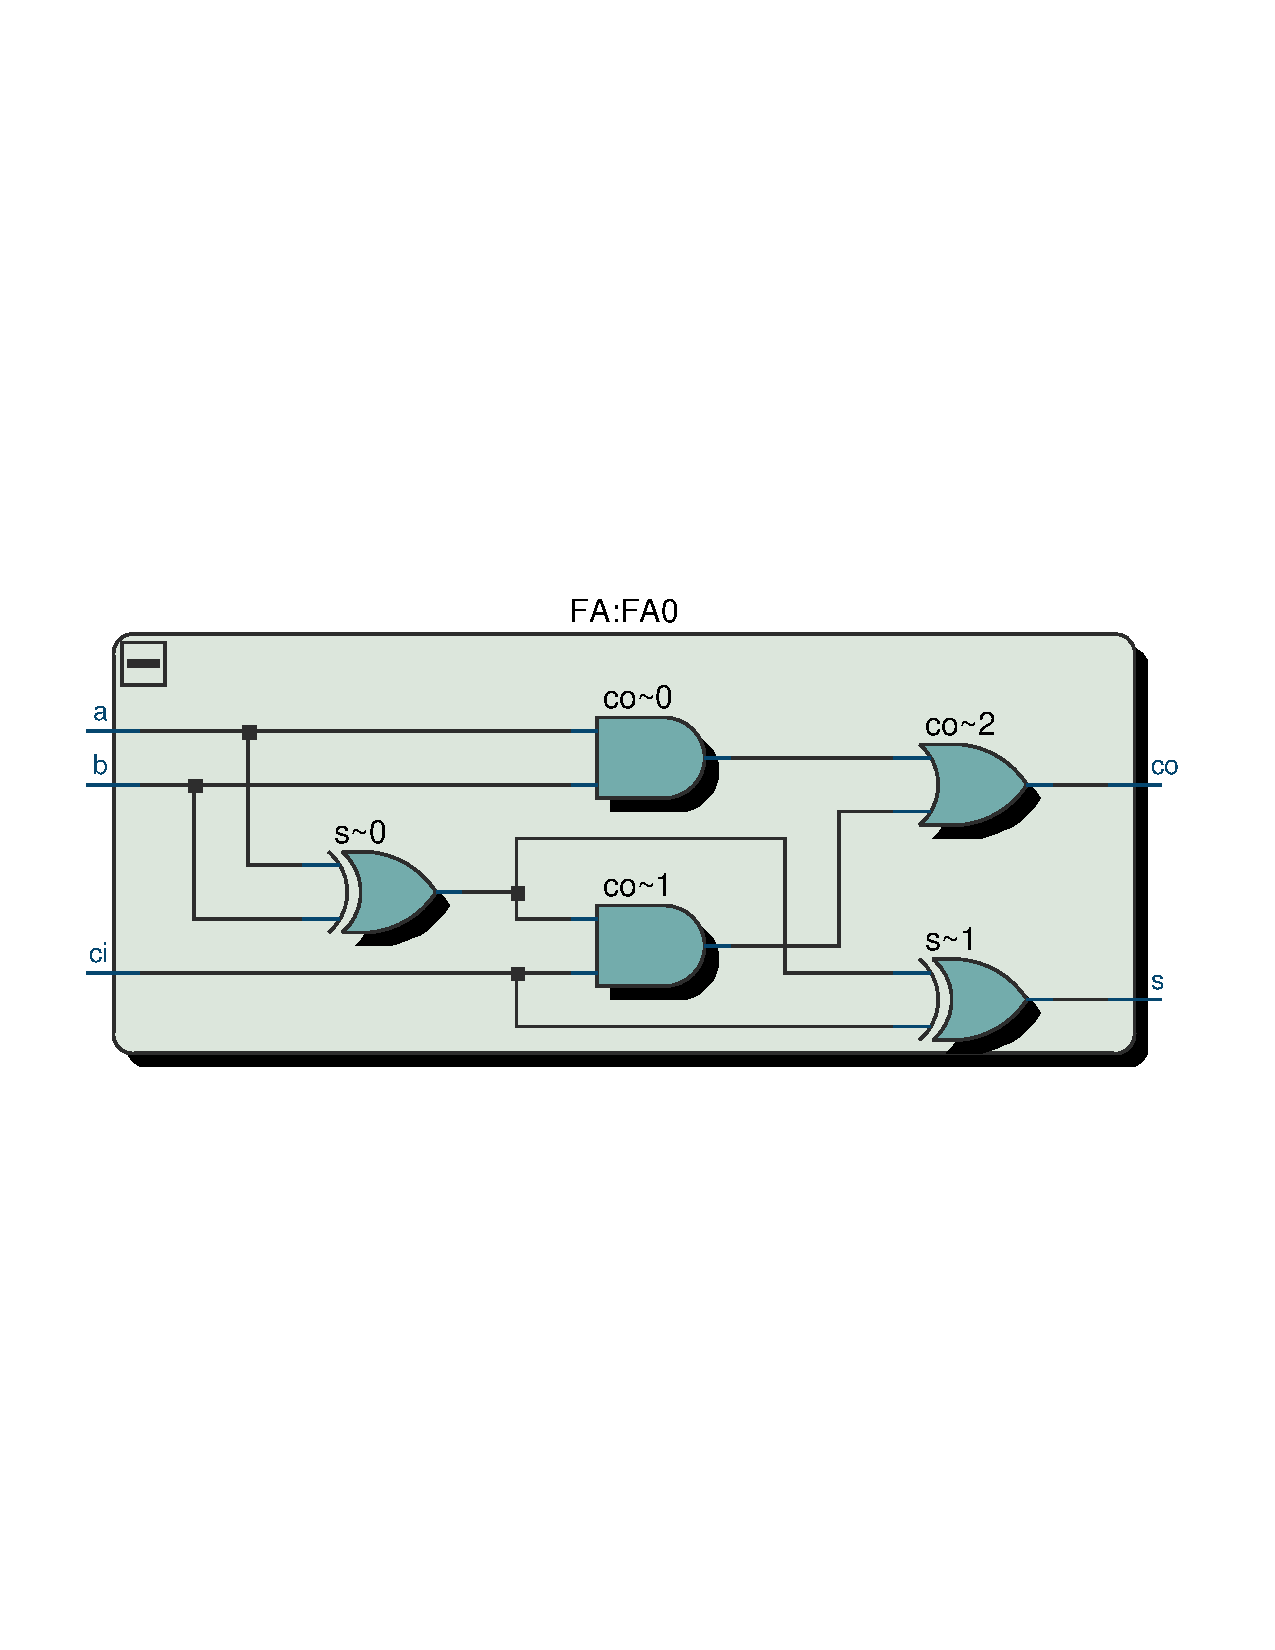
\includegraphics[scale=0.5, clip, trim={0cm 10cm 0cm 10.6cm}]{images/Exc1_FA_RTL.pdf}
\caption*{Full adder}
\end{figure}

\begin{figure}[H]
\centering
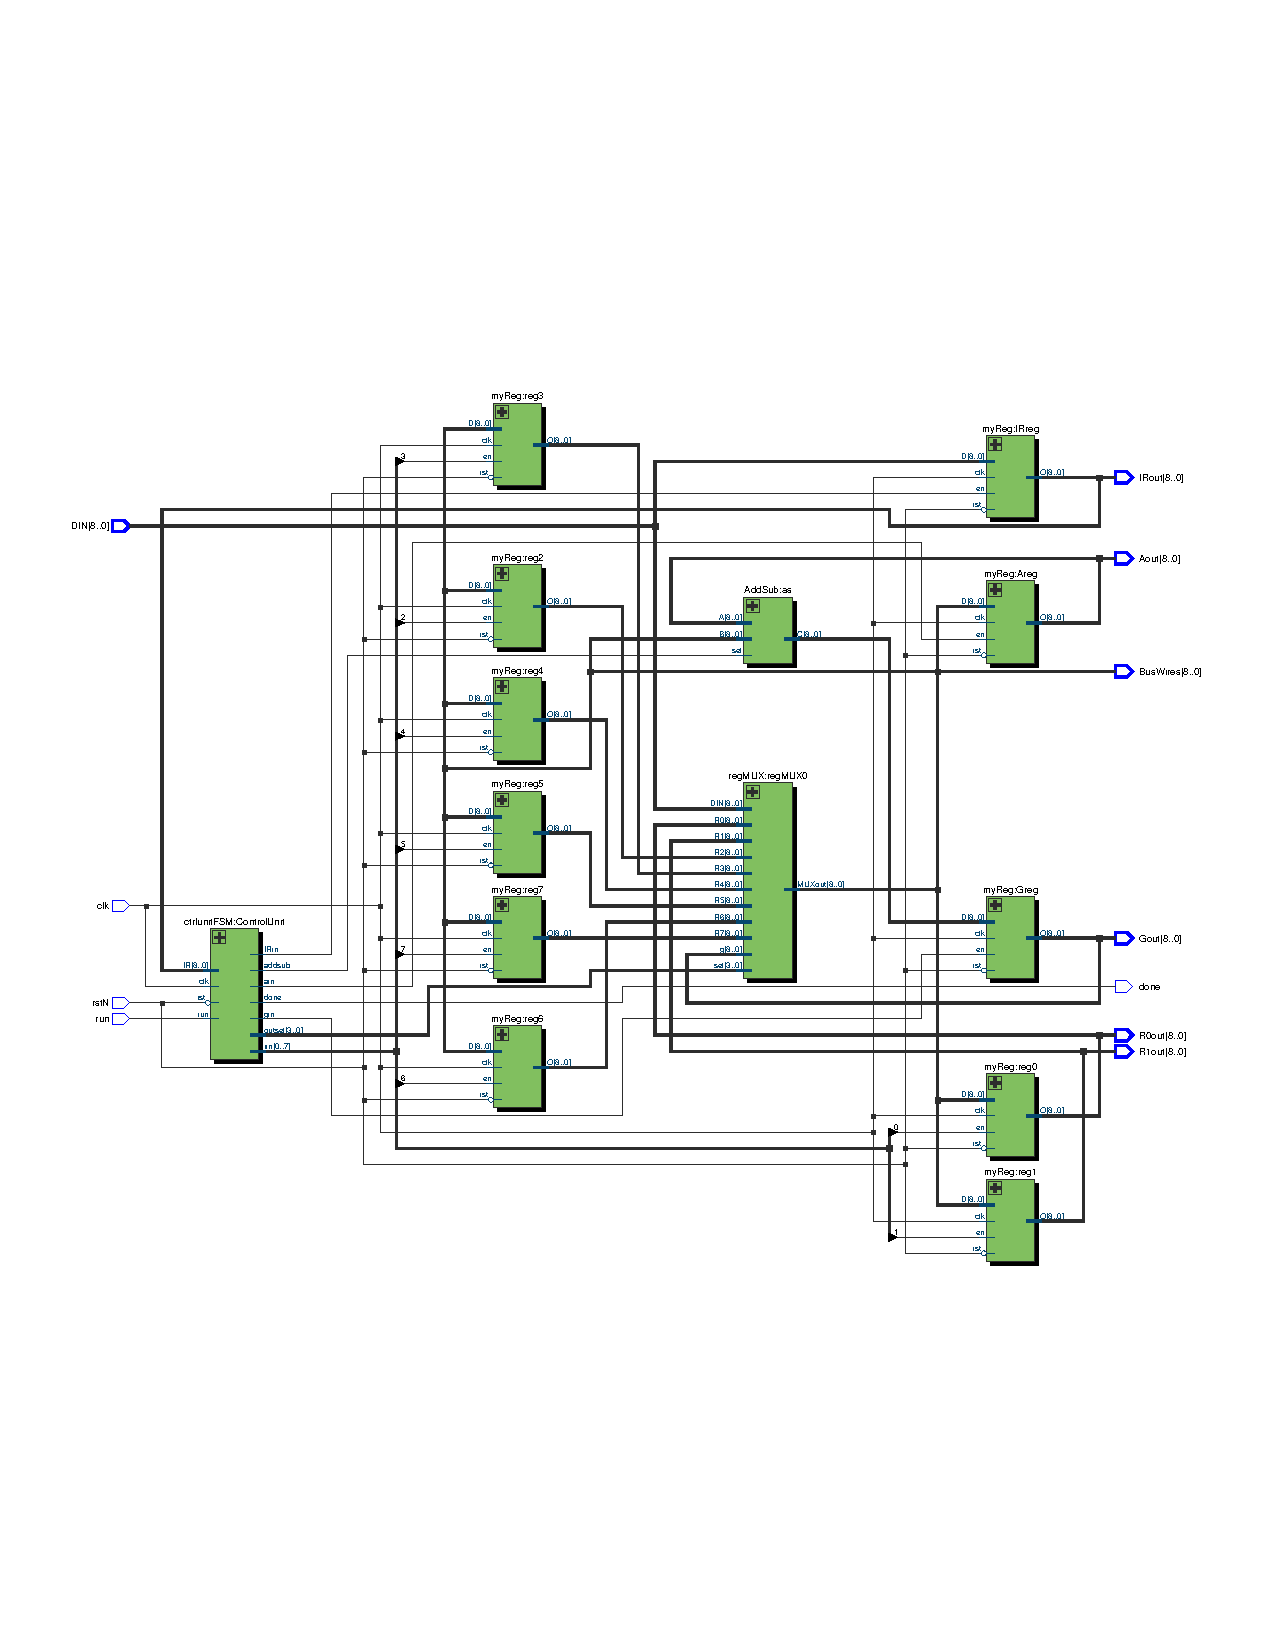
\includegraphics[scale=0.6, clip, trim={0cm 8cm 0cm 9cm}]{images/Exc1_RTL.pdf}
\caption*{Top level}
\end{figure}

\section{Known how to program BCD adder}
\begin{minipage}[t]{0.4\textwidth}
{\bf \normalsize Comparator $>9$}
\begin{table}[H]
\centering
\begin{tabular}{ccccc|c}
$v_4$&$v_3$&$v_2$&$v_1$&$v_0$&$z$\\
\hline
$0$&$0$&$0$&$0$&$0$&$0$\\
$0$&$0$&$0$&$0$&$1$&$0$\\
$0$&$0$&$0$&$1$&$0$&$0$\\
$0$&$0$&$0$&$1$&$1$&$0$\\
$0$&$0$&$1$&$0$&$0$&$0$\\
$0$&$0$&$1$&$0$&$1$&$0$\\
$0$&$0$&$1$&$1$&$0$&$0$\\
$0$&$0$&$1$&$1$&$1$&$0$\\
$0$&$1$&$0$&$0$&$0$&$0$\\
$0$&$1$&$0$&$0$&$1$&$0$\\
$0$&$1$&$0$&$1$&$0$&$1$\\
$0$&$1$&$0$&$1$&$1$&$1$\\
$0$&$1$&$1$&$0$&$0$&$1$\\
$0$&$1$&$1$&$0$&$1$&$1$\\
$0$&$1$&$1$&$1$&$0$&$1$\\
$0$&$1$&$1$&$1$&$1$&$1$\\
$1$&$0$&$0$&$0$&$0$&$1$\\
$1$&$0$&$0$&$0$&$1$&$1$\\
$1$&$0$&$0$&$1$&$0$&$1$\\
$1$&$0$&$0$&$1$&$1$&$1$\\
$1$&$0$&$1$&$0$&$0$&$1$\\
$1$&$0$&$1$&$0$&$1$&$1$\\
$1$&$0$&$1$&$1$&$0$&$1$\\
$1$&$0$&$1$&$1$&$1$&$1$\\
$1$&$1$&$0$&$0$&$0$&$1$\\
$1$&$1$&$0$&$0$&$1$&$1$\\
$1$&$1$&$0$&$1$&$0$&$1$\\
$1$&$1$&$0$&$1$&$1$&$1$\\
$1$&$1$&$1$&$0$&$0$&$1$\\
$1$&$1$&$1$&$0$&$1$&$1$\\
$1$&$1$&$1$&$1$&$0$&$1$\\
$1$&$1$&$1$&$1$&$1$&$1$
\end{tabular}

$\Rightarrow z=v_3(v_2+v_1)$
\end{table}
\end{minipage}
\begin{minipage}[t]{0.6\textwidth}
{\bf \normalsize Circuit A}
\begin{table}[H]
\centering
\begin{tabular}{ccccc|ccccc}
$v_4$&$v_3$&$v_2$&$v_1$&$v_0$&$A_4$&$A_3$&$A_2$&$A_1$&$A_0$\\
\hline
$0$&$0$&$0$&$0$&$0$&$\times$&$\times$&$\times$&$\times$&$\times$\\
$0$&$0$&$0$&$0$&$1$&$\times$&$\times$&$\times$&$\times$&$\times$\\
$0$&$0$&$0$&$1$&$0$&$\times$&$\times$&$\times$&$\times$&$\times$\\
$0$&$0$&$0$&$1$&$1$&$\times$&$\times$&$\times$&$\times$&$\times$\\
$0$&$0$&$1$&$0$&$0$&$\times$&$\times$&$\times$&$\times$&$\times$\\
$0$&$0$&$1$&$0$&$1$&$\times$&$\times$&$\times$&$\times$&$\times$\\
$0$&$0$&$1$&$1$&$0$&$\times$&$\times$&$\times$&$\times$&$\times$\\
$0$&$0$&$1$&$1$&$1$&$\times$&$\times$&$\times$&$\times$&$\times$\\
$0$&$1$&$0$&$0$&$0$&$\times$&$\times$&$\times$&$\times$&$\times$\\
$0$&$1$&$0$&$0$&$1$&$\times$&$\times$&$\times$&$\times$&$\times$\\
$0$&$1$&$0$&$1$&$0$&$0$&$0$&$0$&$0$&$0$\\
$0$&$1$&$0$&$1$&$1$&$0$&$0$&$0$&$0$&$1$\\
$0$&$1$&$1$&$0$&$0$&$0$&$0$&$0$&$1$&$0$\\
$0$&$1$&$1$&$0$&$1$&$0$&$0$&$0$&$1$&$1$\\
$0$&$1$&$1$&$1$&$0$&$0$&$0$&$1$&$0$&$0$\\
$0$&$1$&$1$&$1$&$1$&$0$&$0$&$1$&$0$&$1$\\
$1$&$0$&$0$&$0$&$0$&$0$&$0$&$1$&$1$&$0$\\
$1$&$0$&$0$&$0$&$1$&$0$&$0$&$1$&$1$&$1$\\
$1$&$0$&$0$&$1$&$0$&$0$&$1$&$0$&$0$&$0$\\
$1$&$0$&$0$&$1$&$1$&$0$&$1$&$0$&$0$&$1$\\
$1$&$0$&$1$&$0$&$0$&$\times$&$\times$&$\times$&$\times$&$\times$\\
$1$&$0$&$1$&$0$&$1$&$\times$&$\times$&$\times$&$\times$&$\times$\\
$1$&$0$&$1$&$1$&$0$&$\times$&$\times$&$\times$&$\times$&$\times$\\
$1$&$0$&$1$&$1$&$1$&$\times$&$\times$&$\times$&$\times$&$\times$\\
$1$&$1$&$0$&$0$&$0$&$\times$&$\times$&$\times$&$\times$&$\times$\\
$1$&$1$&$0$&$0$&$1$&$\times$&$\times$&$\times$&$\times$&$\times$\\
$1$&$1$&$0$&$1$&$0$&$\times$&$\times$&$\times$&$\times$&$\times$\\
$1$&$1$&$0$&$1$&$1$&$\times$&$\times$&$\times$&$\times$&$\times$\\
$1$&$1$&$1$&$0$&$0$&$\times$&$\times$&$\times$&$\times$&$\times$\\
$1$&$1$&$1$&$0$&$1$&$\times$&$\times$&$\times$&$\times$&$\times$\\
$1$&$1$&$1$&$1$&$0$&$\times$&$\times$&$\times$&$\times$&$\times$\\
$1$&$1$&$1$&$1$&$1$&$\times$&$\times$&$\times$&$\times$&$\times$\\
\end{tabular}

$\Rightarrow \begin{array}{rcl}
A_4 & = & 0 \\
A_3 & = & \overline v_3 v_1 \\
A_2 & = & \overline{v_2 \oplus v_1} \\
A_1 & = & \bar v_1\\
A_0 & = & v_0
\end{array}$
\end{table}
\end{minipage}

\subsection{Code}

\subsubsection{MUX.vhd}
\begin{minted}{vhdl}
LIBRARY ieee;
USE ieee.std_logic_1164.ALL;

ENTITY MUX IS
	PORT (
		muxIn1 : IN STD_LOGIC;
		muxSel : IN STD_LOGIC;
		muxIn2 : IN STD_LOGIC;
		muxOut : OUT STD_LOGIC
	);
END ENTITY;
ARCHITECTURE arch OF MUX IS
BEGIN
	muxOut <= (NOT(muxSel) AND muxIn1) OR (muxSel AND muxIn2);
END arch;
\end{minted}

\subsubsection{FourBitMUX.vhd}
\begin{minted}{vhdl}
LIBRARY ieee;
USE ieee.std_logic_1164.ALL;

ENTITY FourBitMUX IS
	PORT (
		fourBitMuxIn1 : IN STD_LOGIC_VECTOR(4 DOWNTO 0);
		fourBitMuxIn2 : IN STD_LOGIC_VECTOR(4 DOWNTO 0);
		fourBitMuxSel : IN STD_LOGIC;
		fourBitMuxOut : OUT STD_LOGIC_VECTOR(4 DOWNTO 0)
	);
END ENTITY;

ARCHITECTURE arch OF FourBitMUX IS
	COMPONENT MUX
		PORT (
			muxIn1 : IN STD_LOGIC;
			muxSel : IN STD_LOGIC;
			muxIn2 : IN STD_LOGIC;
			muxOut : OUT STD_LOGIC
		);
	END COMPONENT;
BEGIN
	gen : FOR i IN 4 DOWNTO 0 GENERATE
		MUX2 : MUX PORT MAP(
			muxSel => fourBitMuxSel,
			muxIn1 => fourBitMuxIn1(i),
			muxIn2 => fourBitMuxIn2(i),
			muxOut => fourBitMuxOut(i)
		);
	END GENERATE;
END arch;
\end{minted}

\subsubsection{Comparator.vhd}
\begin{minted}{vhdl}
LIBRARY ieee;
USE ieee.std_logic_1164.ALL;

ENTITY Comparator IS
	PORT (
		compIn : IN STD_LOGIC_VECTOR(4 DOWNTO 0);
		compOut : OUT STD_LOGIC
	);
END ENTITY;

ARCHITECTURE behave OF Comparator IS
BEGIN
	-- Z = A+B(C+D)
	compOut <= compIn(4) OR (compIn(3) AND (compIn(2) OR compIn(1)));

END ARCHITECTURE;
\end{minted}

\subsubsection{CircuitA.vhd}
\begin{minted}{vhdl}
LIBRARY ieee;
USE ieee.std_logic_1164.ALL;

ENTITY CircuitA IS
	PORT (
		dIn : IN STD_LOGIC_VECTOR(4 DOWNTO 0);
		dOut : OUT STD_LOGIC_VECTOR(4 DOWNTO 0)
	);
END ENTITY;

ARCHITECTURE behave OF CircuitA IS
BEGIN
	-- V = 0
	dOut(4) <= '0';

	-- W = B'*D
	dOut(3) <= NOT(dIn(3)) AND dIn(1);

	-- Y = C'D' + CD
	dOut(2) <= dIn(2) XNOR dIn(1);

	-- X = D'
	dOut(1) <= NOT(dIn(1));

	-- Z = E
	dOut(0) <= dIn(0);

END ARCHITECTURE;
\end{minted}

\subsubsection{BCD.vhd}
\begin{minted}{vhdl}
LIBRARY ieee;
USE ieee.std_logic_1164.ALL;

ENTITY BCD IS
	PORT (
		c : IN STD_LOGIC_VECTOR(4 DOWNTO 0);
		HEXn : OUT STD_LOGIC_VECTOR(0 TO 6)
	);
END BCD;

ARCHITECTURE behavior OF BCD IS
	SIGNAL HEX : STD_LOGIC_VECTOR(0 TO 6);
BEGIN
	HEXn <= NOT(HEX);
	WITH c SELECT
		HEX <= "1111110" WHEN "00000",
		"0110000" WHEN "00001",
		"1101101" WHEN "00010",
		"1111001" WHEN "00011",
		"0110011" WHEN "00100",
		"1011011" WHEN "00101",
		"1011111" WHEN "00110",
		"1110000" WHEN "00111",
		"1111111" WHEN "01000",
		"1111011" WHEN "01001",
		"0000000" WHEN OTHERS;
END behavior;
\end{minted}

\subsubsection{BCDDisplay.vhd}
\begin{minted}{vhdl}
LIBRARY ieee;
USE ieee.std_logic_1164.ALL;

ENTITY BCDDisplay IS
	PORT (
		V : IN STD_LOGIC_VECTOR(4 DOWNTO 0);
		HEX0 : OUT STD_LOGIC_VECTOR(0 TO 6);
		HEX1 : OUT STD_LOGIC_VECTOR(0 TO 6)
	);
END ENTITY;

ARCHITECTURE behave OF BCDDisplay IS

	SIGNAL z : STD_LOGIC;
	SIGNAL A, m : STD_LOGIC_VECTOR(4 DOWNTO 0);

	COMPONENT FourBitMUX IS
		PORT (
			fourBitMuxIn1 : IN STD_LOGIC_VECTOR(4 DOWNTO 0);
			fourBitMuxIn2 : IN STD_LOGIC_VECTOR(4 DOWNTO 0);
			fourBitMuxSel : IN STD_LOGIC;
			fourBitMuxOut : OUT STD_LOGIC_VECTOR(4 DOWNTO 0)
		);
	END COMPONENT;

	COMPONENT Comparator IS
		PORT (
			compIn : IN STD_LOGIC_VECTOR(4 DOWNTO 0);
			compOut : OUT STD_LOGIC
		);
	END COMPONENT;

	COMPONENT CircuitA IS
		PORT (
			dIn : IN STD_LOGIC_VECTOR(4 DOWNTO 0);
			dOut : OUT STD_LOGIC_VECTOR(4 DOWNTO 0)
		);
	END COMPONENT;

	COMPONENT BCD IS
		PORT (
			c : IN STD_LOGIC_VECTOR(4 DOWNTO 0);
			HEXn : OUT STD_LOGIC_VECTOR(0 TO 6)
		);
	END COMPONENT;
BEGIN
	comp : Comparator PORT MAP(
		compIn => V,
		compOut => z
	);

	cirA : CircuitA PORT MAP(
		dIn => V,
		dOut => A
	);

	mux : FourBitMUX PORT MAP(
		fourBitMuxIn1 => V,
		fourBitMuxIn2 => A,
		fourBitMuxSel => z,
		fourBitMuxOut => m
	);

	HEX01 : BCD PORT MAP(c => "0000" & z, HEXn => HEX1);
	HEX00 : BCD PORT MAP(c => m, HEXn => HEX0);

END ARCHITECTURE;
\end{minted}

\subsubsection{FA.vhd}
\begin{minted}{vhdl}
LIBRARY ieee;
USE ieee.std_logic_1164.ALL;

ENTITY Exc1 IS
	PORT (
		a : IN STD_LOGIC;
		b : IN STD_LOGIC;
		ci : IN STD_LOGIC;
		s : OUT STD_LOGIC;
		co : OUT STD_LOGIC
	);
END Exc1;

ARCHITECTURE arch OF Exc1 IS
BEGIN
	s <= a XOR b XOR ci;
	co <= (a AND b) OR (ci AND (a XOR b));
END ARCHITECTURE;
\end{minted}

\subsubsection{Exc2.vhd}
\begin{minted}{vhdl}
LIBRARY ieee;
USE ieee.std_logic_1164.ALL;
USE ieee.numeric_std.ALL;

ENTITY Exc2 IS
	PORT (
		an : IN STD_LOGIC_VECTOR(3 DOWNTO 0);
		bn : IN STD_LOGIC_VECTOR(3 DOWNTO 0);
		cin : IN STD_LOGIC;
		HEXo0 : OUT STD_LOGIC_VECTOR(0 TO 6);
		HEXo1 : OUT STD_LOGIC_VECTOR(0 TO 6);
		HEXo3 : OUT STD_LOGIC_VECTOR(0 TO 6);
		HEXo5 : OUT STD_LOGIC_VECTOR(0 TO 6);
		error : OUT STD_LOGIC;
		sum : OUT STD_LOGIC_VECTOR(4 DOWNTO 0)
	);
END ENTITY;

ARCHITECTURE arch OF Exc2 IS
	SIGNAL cn : STD_LOGIC_VECTOR(4 DOWNTO 1);
	SIGNAL sn : STD_LOGIC_VECTOR(4 DOWNTO 0);
	SIGNAL errorA, errorB : STD_LOGIC;
	COMPONENT FA IS
		PORT (
			a : IN STD_LOGIC;
			b : IN STD_LOGIC;
			ci : IN STD_LOGIC;
			s : OUT STD_LOGIC;
			co : OUT STD_LOGIC
		);
	END COMPONENT;

	COMPONENT BCDDisplay IS
		PORT (
			V : IN STD_LOGIC_VECTOR(4 DOWNTO 0);
			HEX0 : OUT STD_LOGIC_VECTOR(0 TO 6);
			HEX1 : OUT STD_LOGIC_VECTOR(0 TO 6)
		);
	END COMPONENT;

	COMPONENT BCD IS
		PORT (
			c : IN STD_LOGIC_VECTOR(4 DOWNTO 0);
			HEXn : OUT STD_LOGIC_VECTOR(0 TO 6)
		);
	END COMPONENT;

	COMPONENT Comparator IS
		PORT (
			compIn : IN STD_LOGIC_VECTOR(4 DOWNTO 0);
			compOut : OUT STD_LOGIC
		);
	END COMPONENT;
BEGIN
	HEX5 : BCD PORT MAP(c => '0' & an, HEXn => HEXo5);
	HEX3 : BCD PORT MAP(c => '0' & bn, HEXn => HEXo3);

	FA0 : FA PORT MAP(
		a => an(0),
		b => bn(0),
		ci => cin,
		s => sn(0),
		co => cn(1)
	);
	gen : FOR i IN 1 TO 3 GENERATE
		FAn : FA PORT MAP(
			a => an(i),
			b => bn(i),
			ci => cn(i),
			s => sn(i),
			co => cn(i + 1)
		);
	END GENERATE;

	sn(4) <= cn(4);
	sum <= sn;

	BCDHEX : BCDDisplay PORT MAP(V => sn, HEX0 => HEXo0, HEX1 => HEXo1);
	errorLED0 : Comparator PORT MAP(compIn => '0' & an, compOut => errorA);
	errorLED1 : Comparator PORT MAP(compIn => '0' & bn, compOut => errorB);

	error <= errorA OR errorB;
END ARCHITECTURE;
\end{minted}

\subsection{Waveform}
\begin{figure}[H]
\centering
\includegraphics[scale=0.7]{images/Exc2_waveform.png}
\end{figure}


\subsection{Result of RTL viewer}
\begin{figure}[H]
\centering
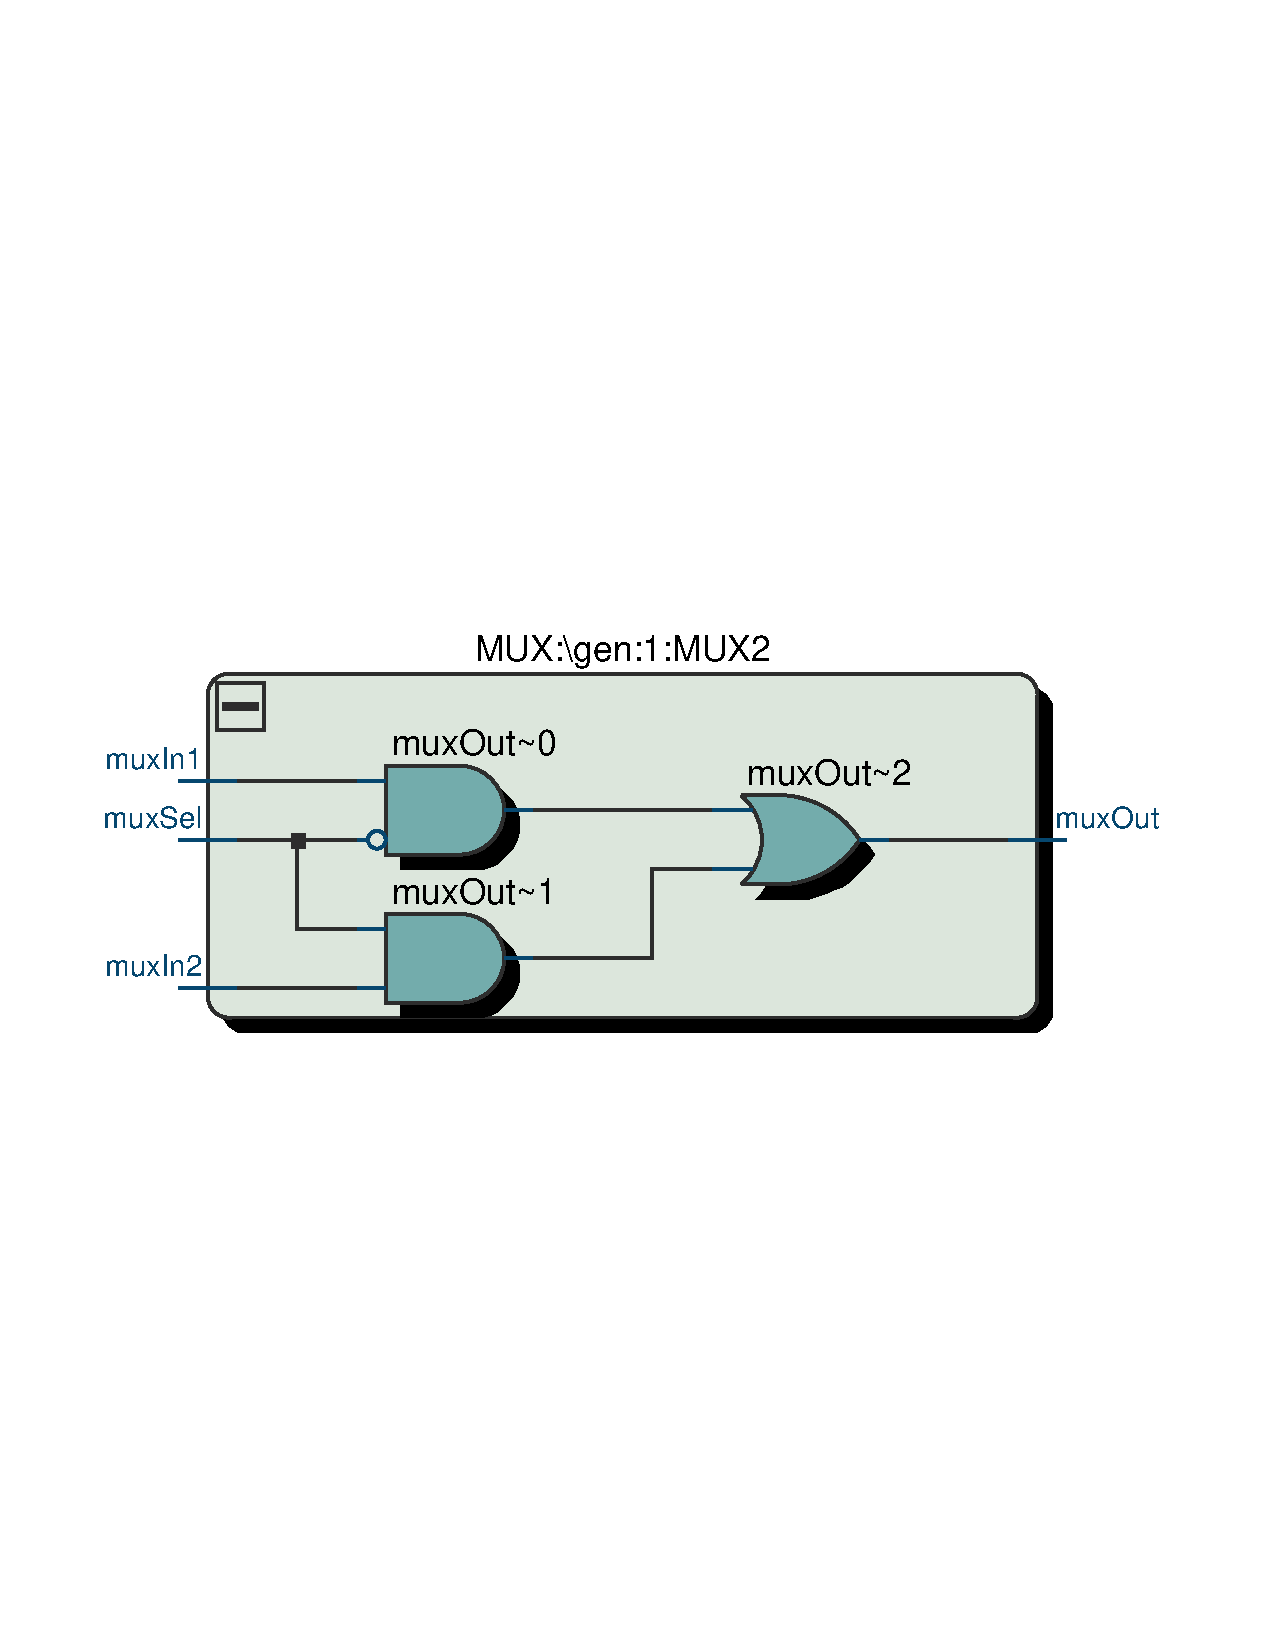
\includegraphics[scale=0.6, clip, trim={0cm 10.2cm 0cm 11.4cm}]{images/Exc2_MUX_RTL.pdf}
\caption*{MUX}
\end{figure}

\begin{figure}[H]
\centering
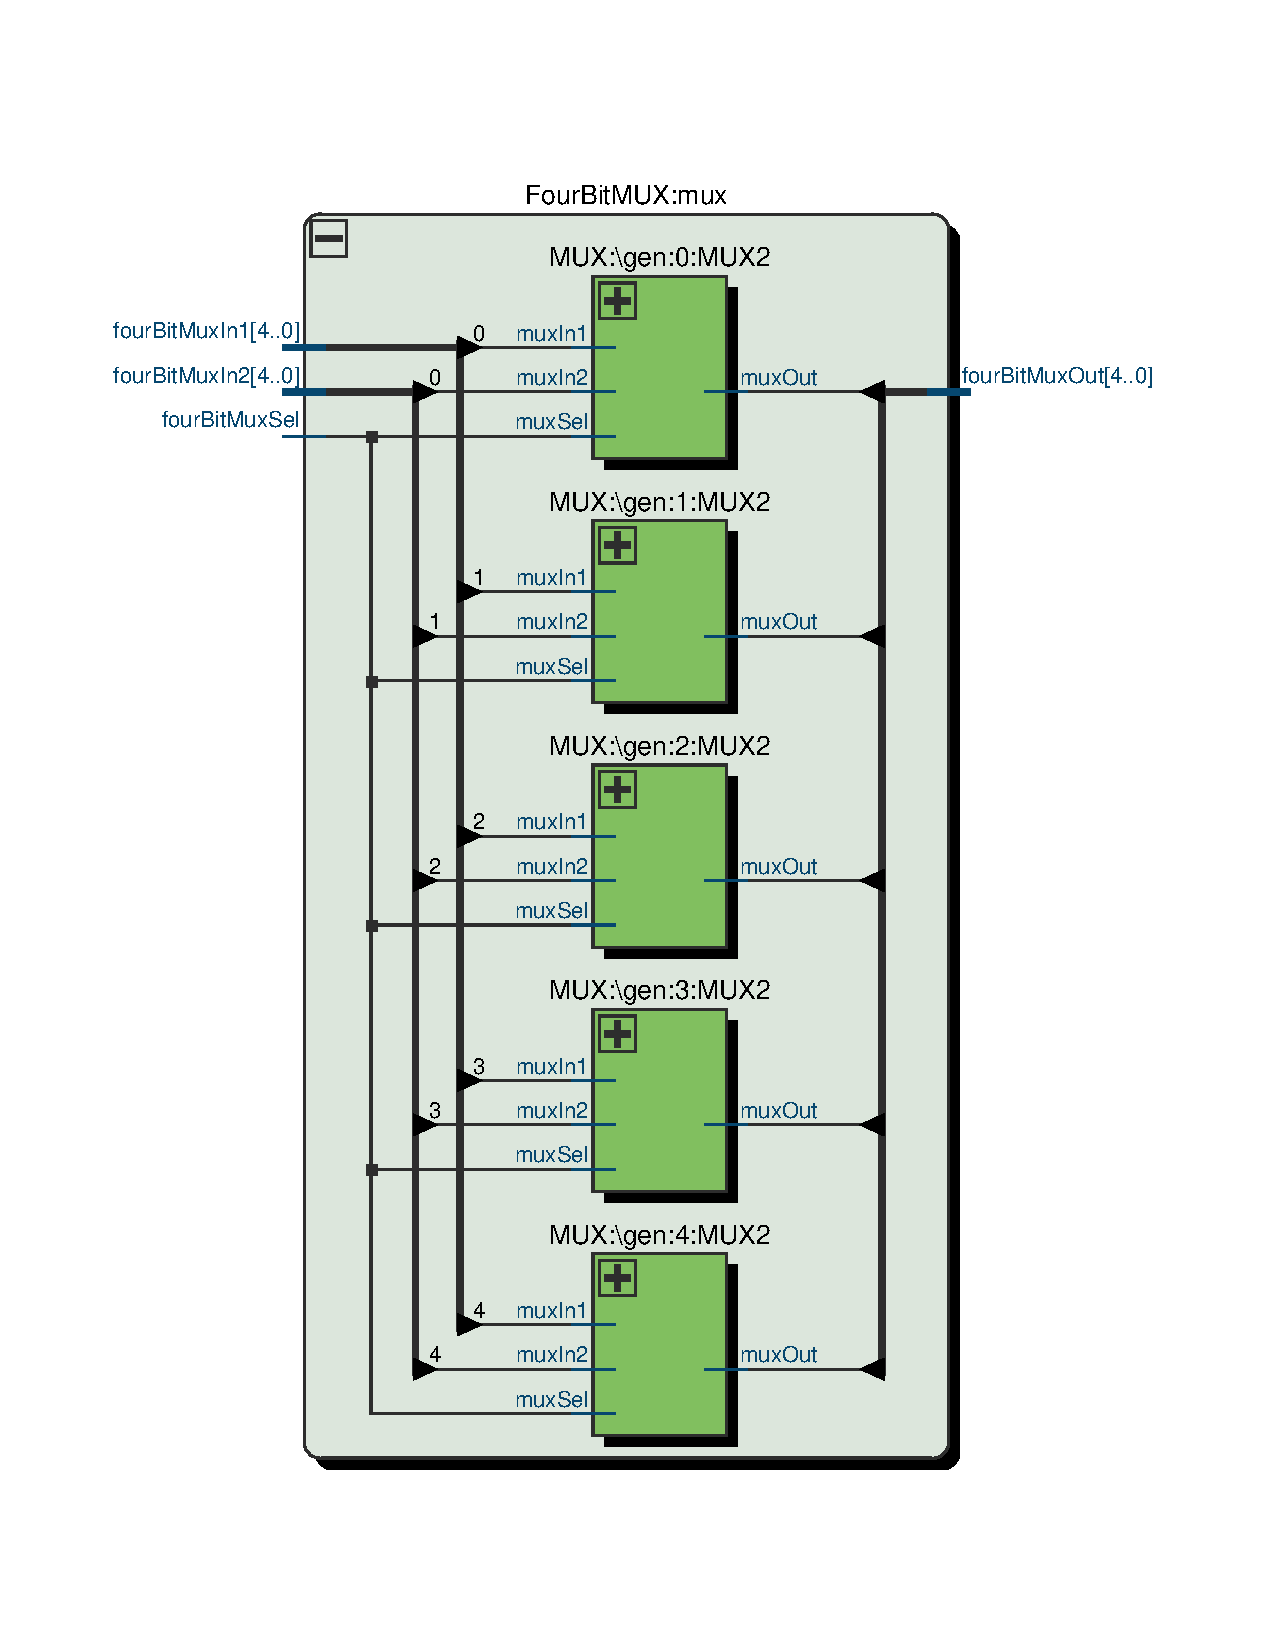
\includegraphics[scale=0.6, clip, trim={0cm 3cm 0cm 3.5cm}]{images/Exc2_FourBitMUX_RTL.pdf}
\caption*{4-bit MUX}
\end{figure}

\begin{figure}[H]
\centering
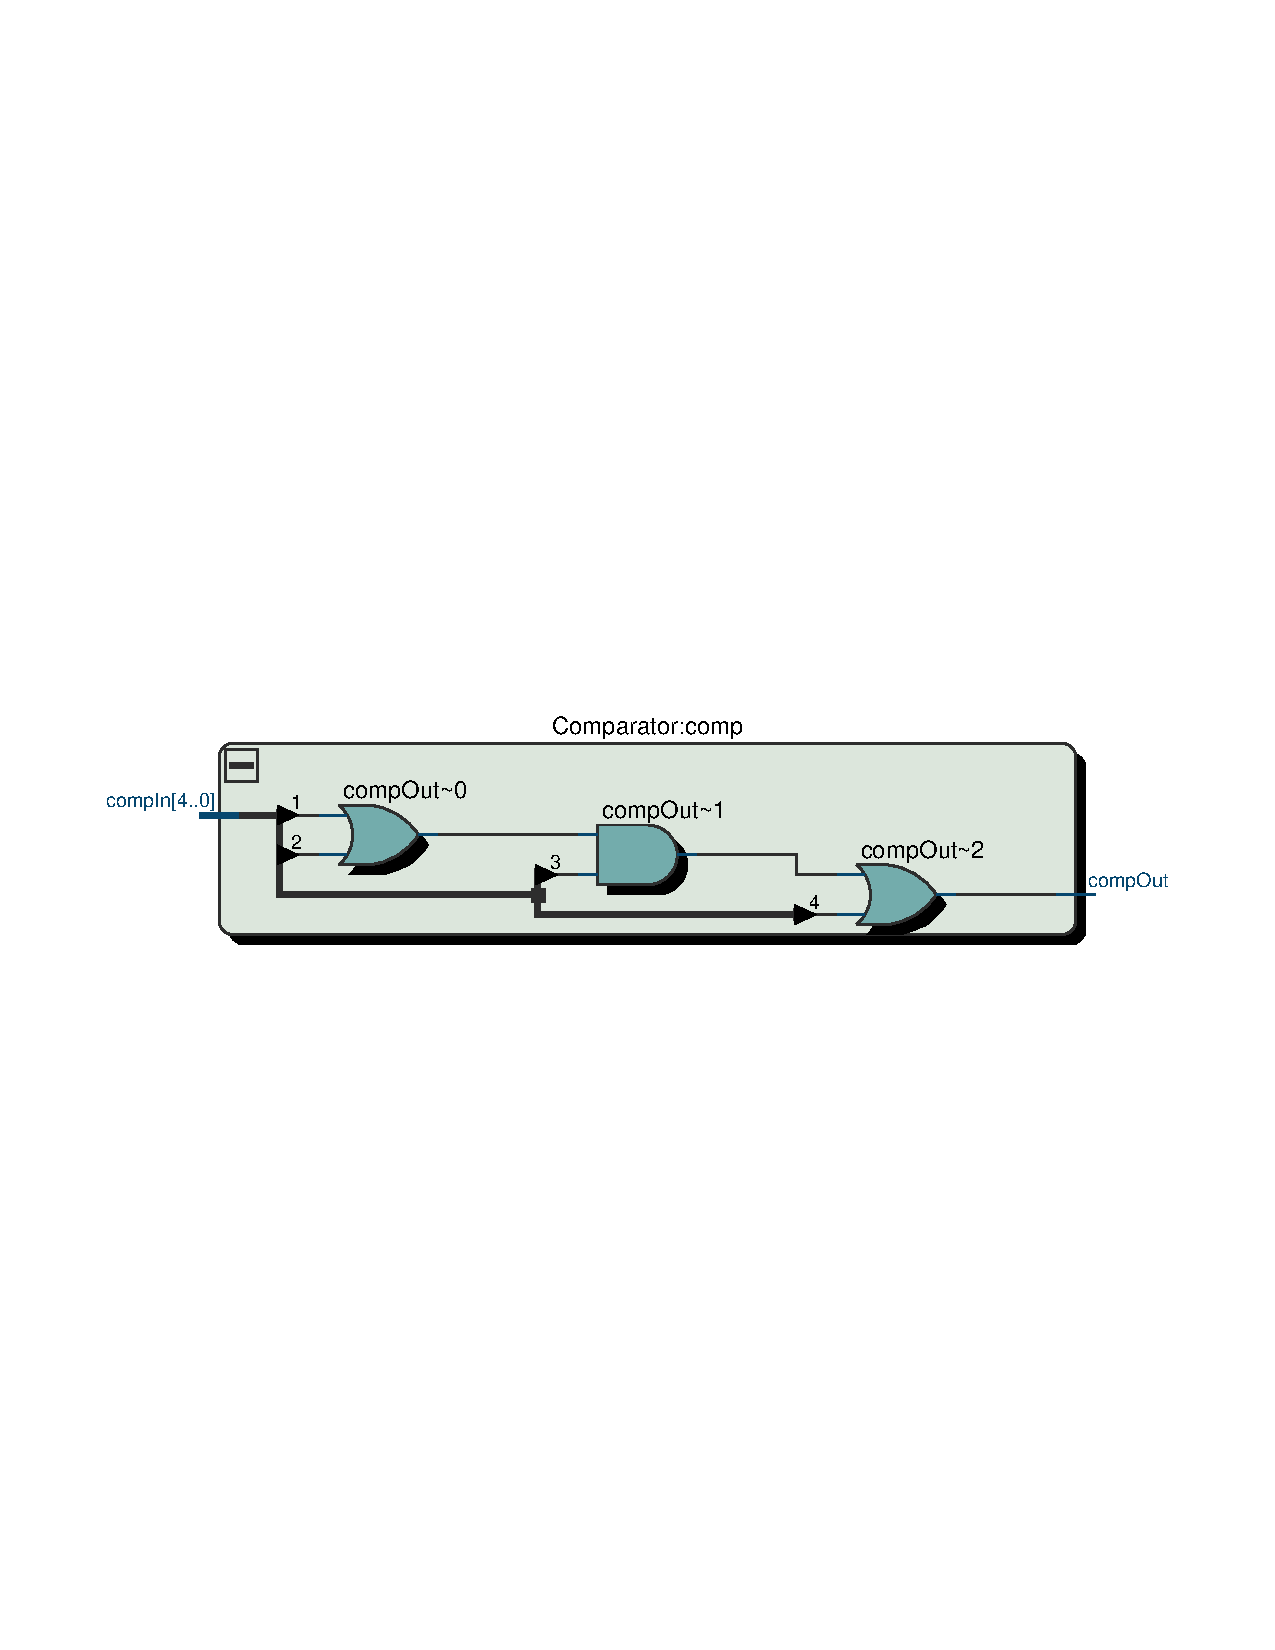
\includegraphics[scale=0.7, clip, trim={0cm 12cm 0cm 12.6cm}]{images/Exc2_Comparator_RTL.pdf}
\caption*{Comparator}
\end{figure}

\begin{figure}[H]
\centering
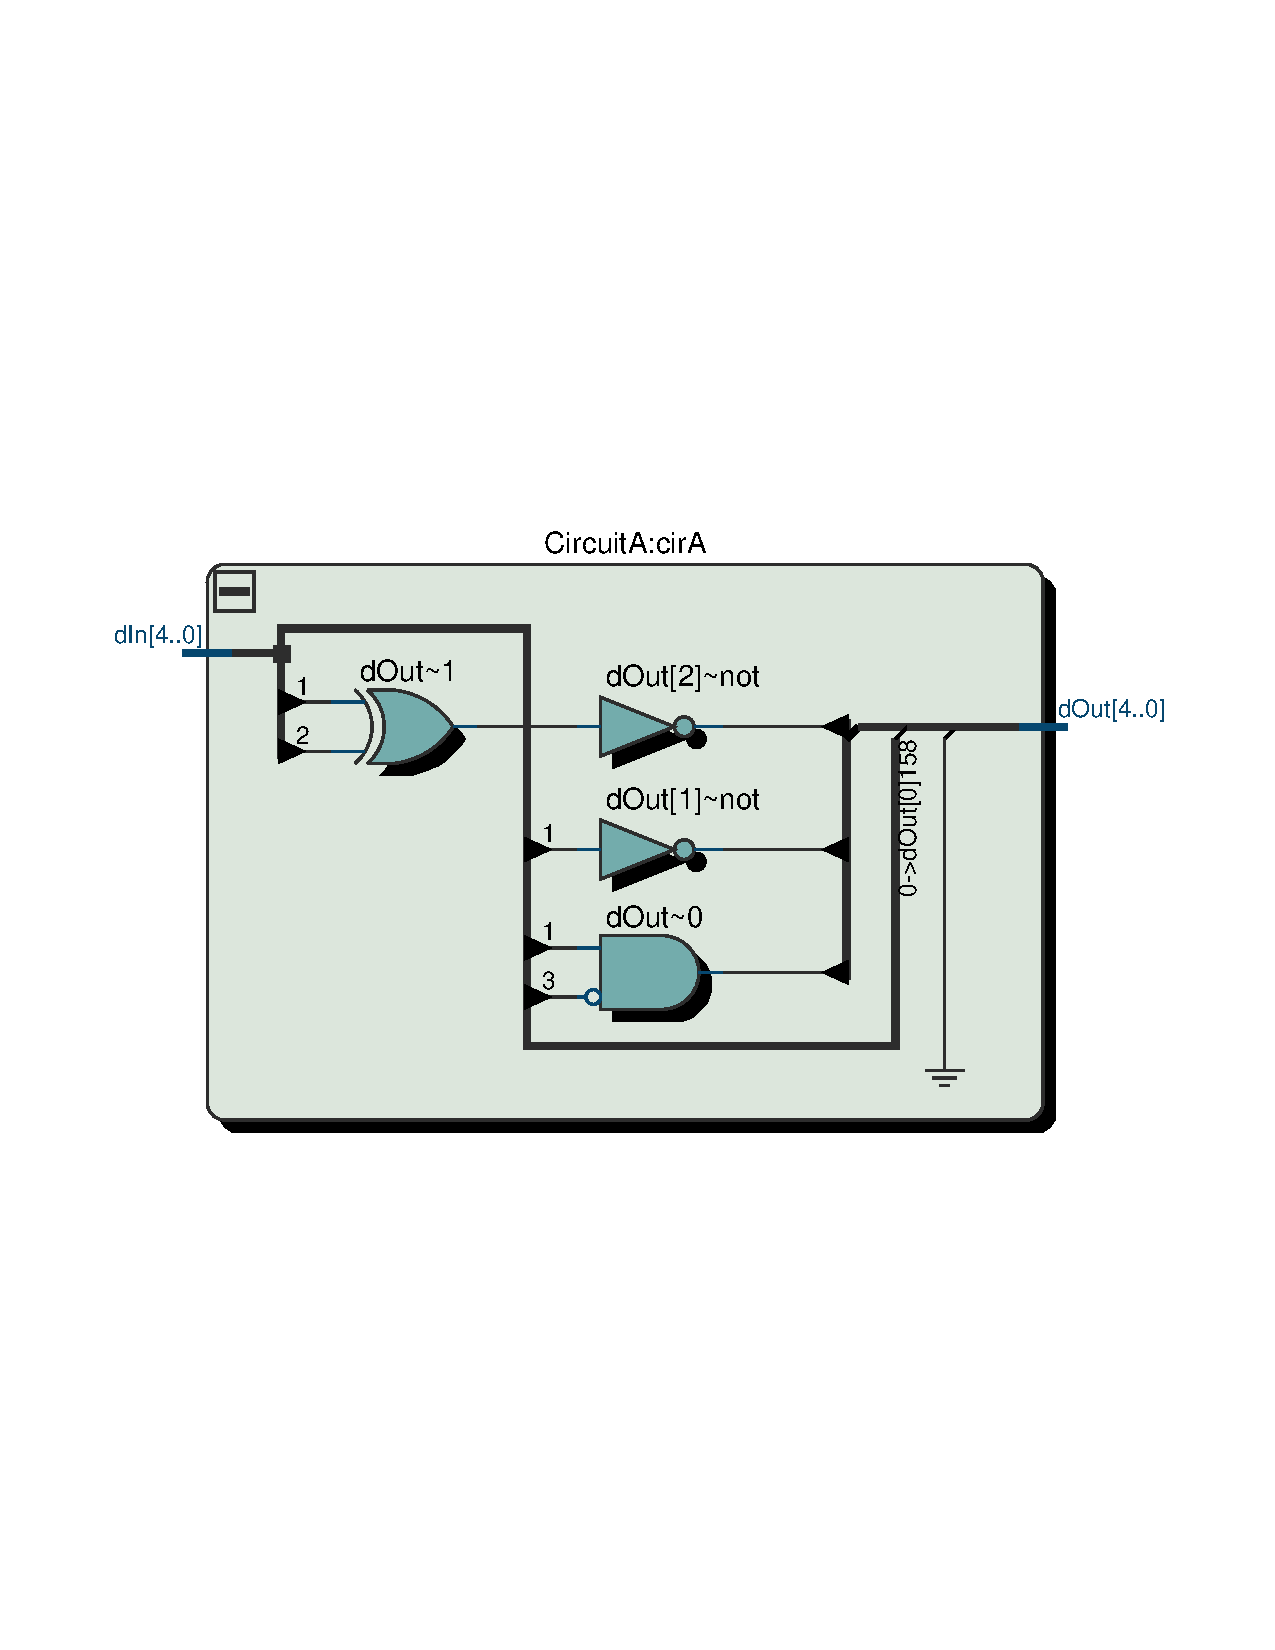
\includegraphics[scale=0.5, clip, trim={0cm 8.5cm 0cm 9.5cm}]{images/Exc2_CircuitA_RTL.pdf}
\caption*{CircuitA}
\end{figure}

\begin{figure}[H]
\centering
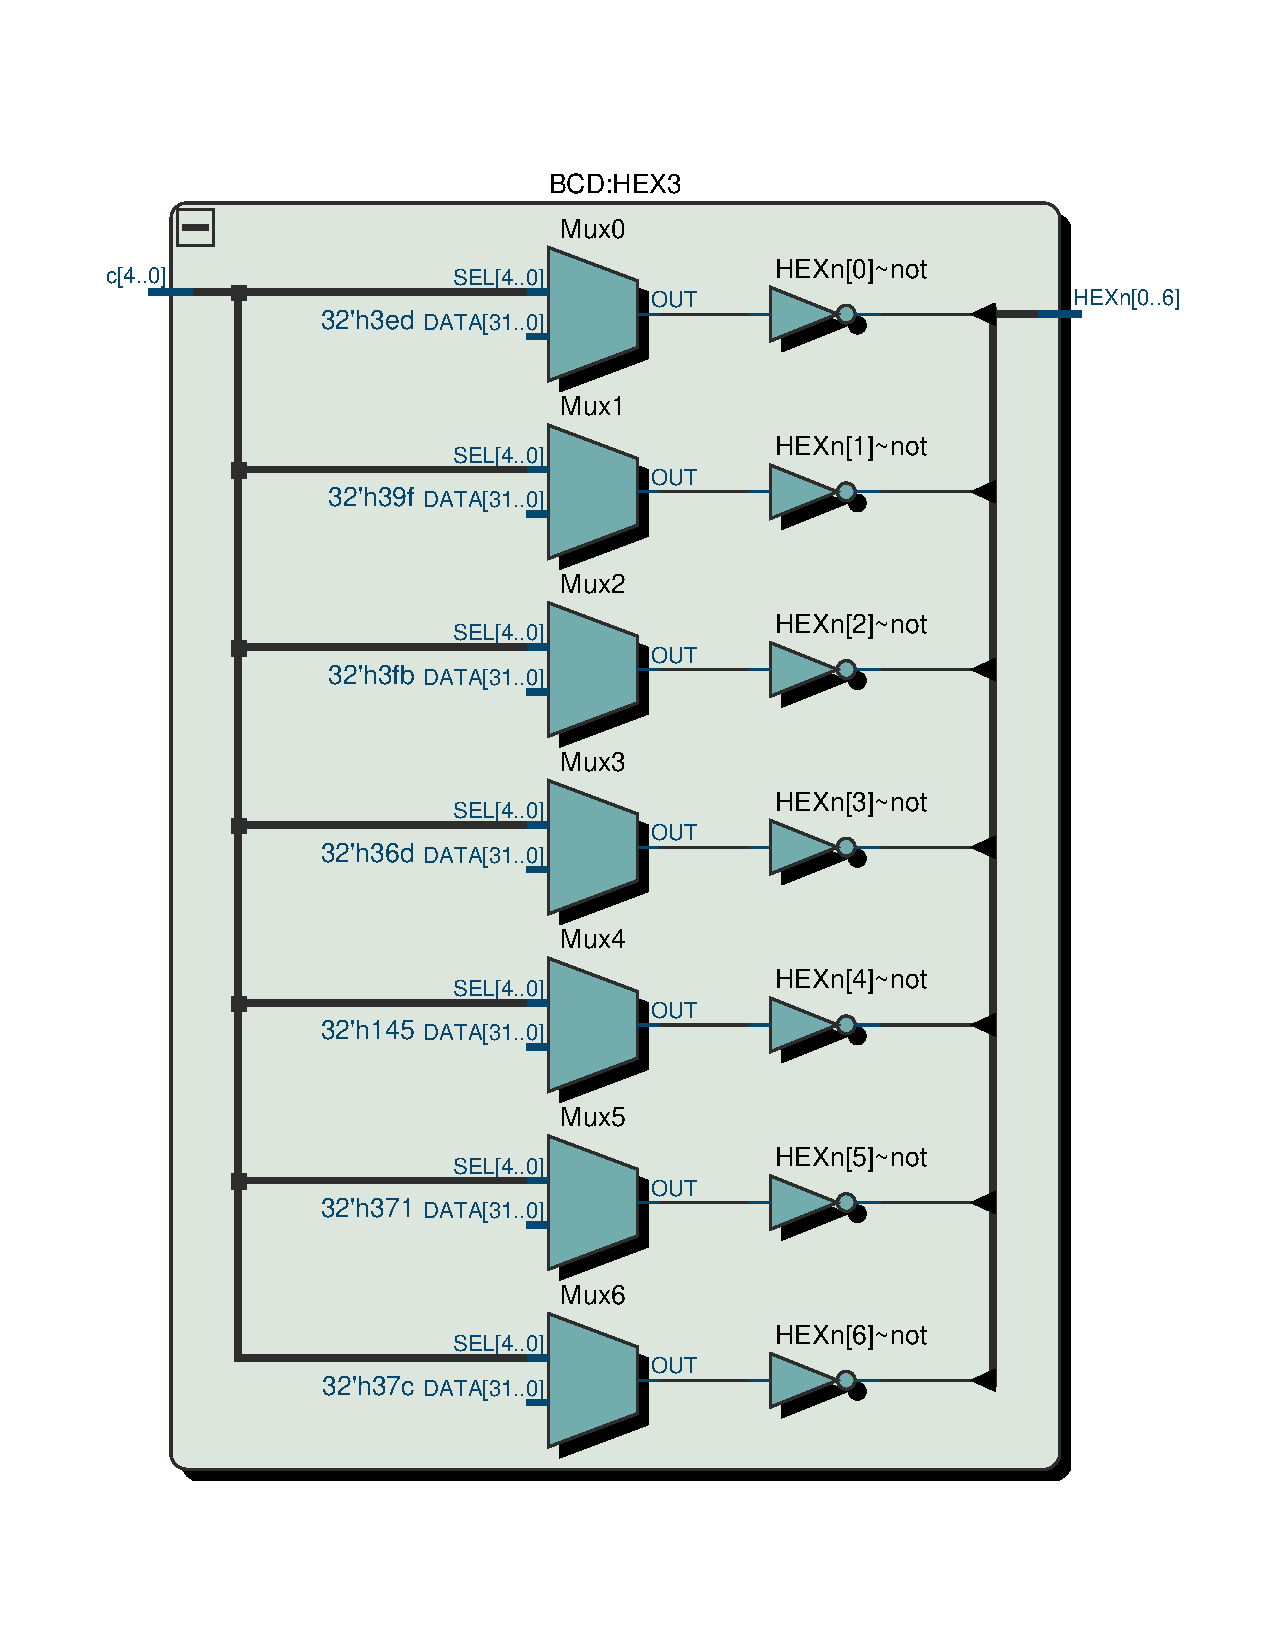
\includegraphics[scale=0.5, clip, trim={0cm 3cm 0cm 3.3cm}]{images/Exc2_BCD_RTL.pdf}
\caption*{BCD MUX}
\end{figure}

\begin{figure}[H]
\centering
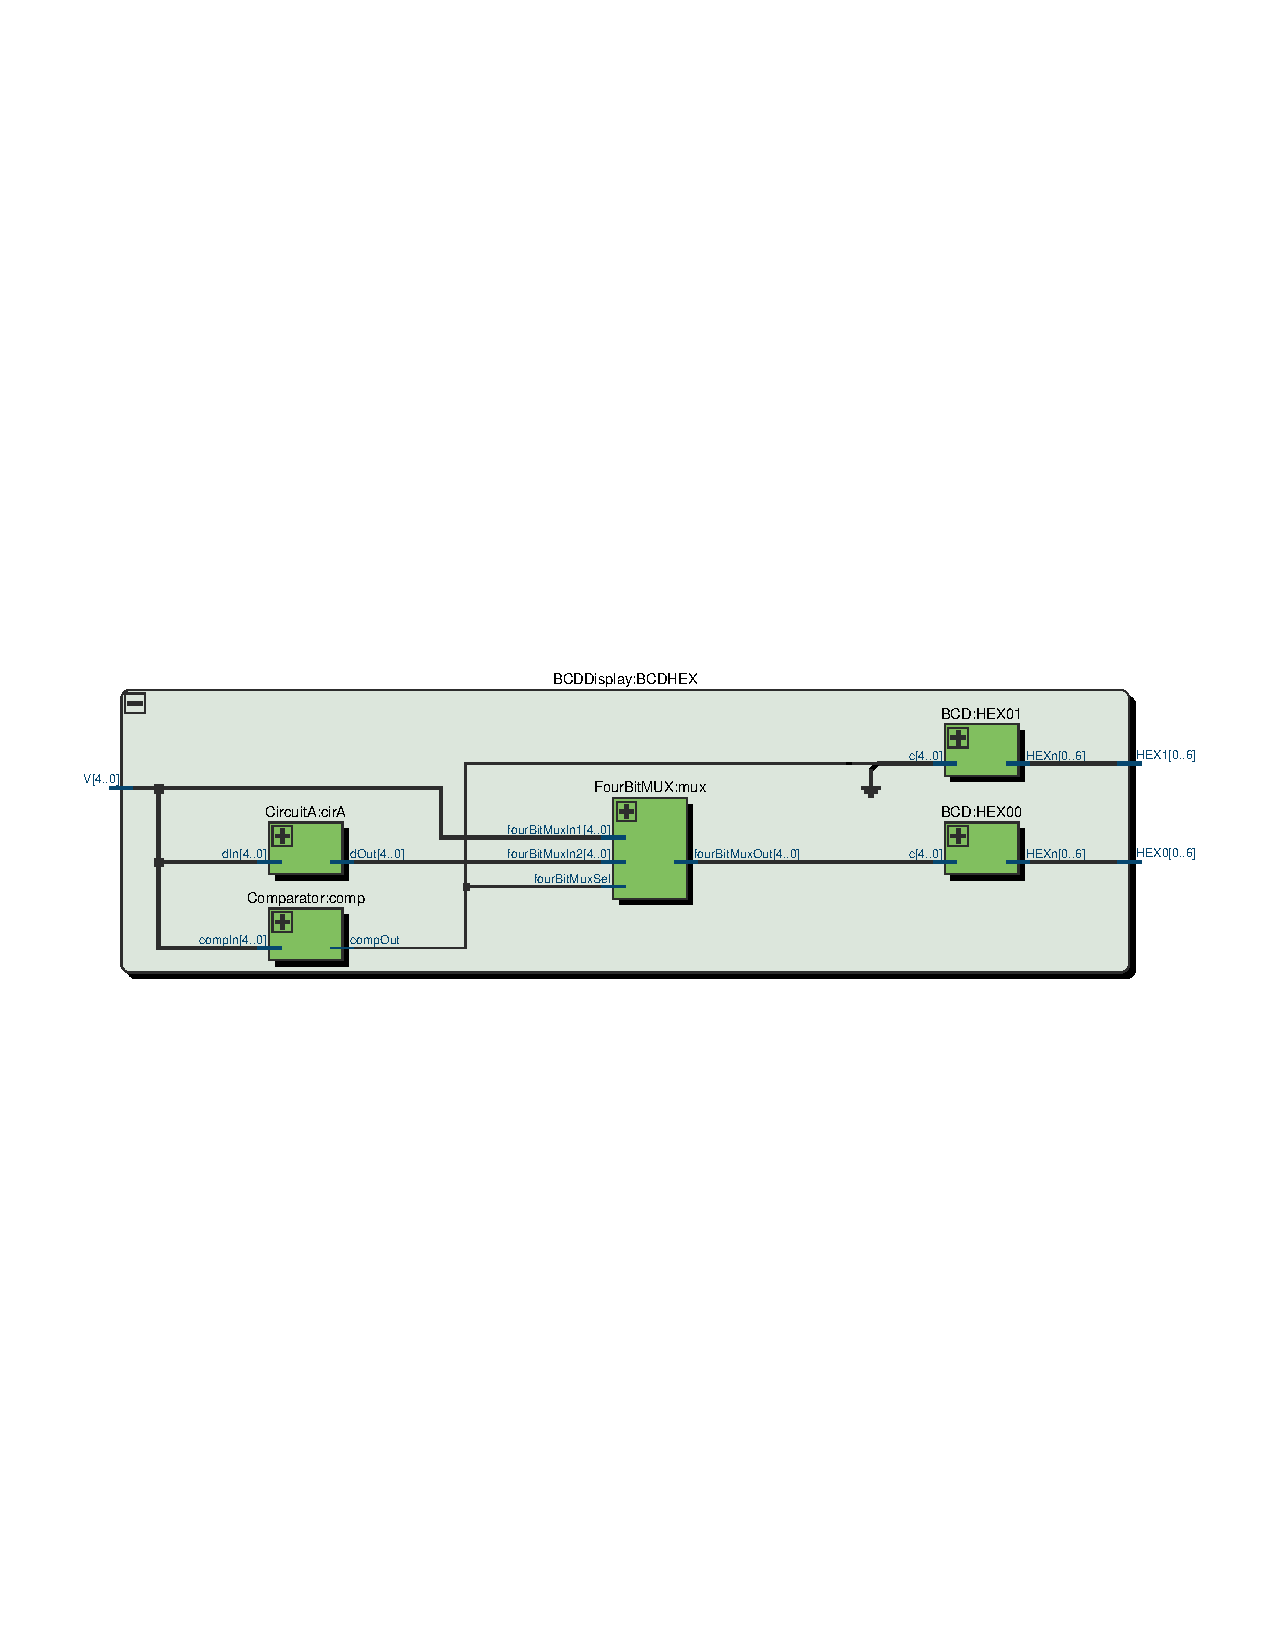
\includegraphics[scale=0.9, clip, trim={0cm 11cm 0cm 11.65cm}]{images/Exc2_BCDDisplay_RTL.pdf}
\caption*{BCD Decoder}
\end{figure}

\begin{figure}[H]
\centering
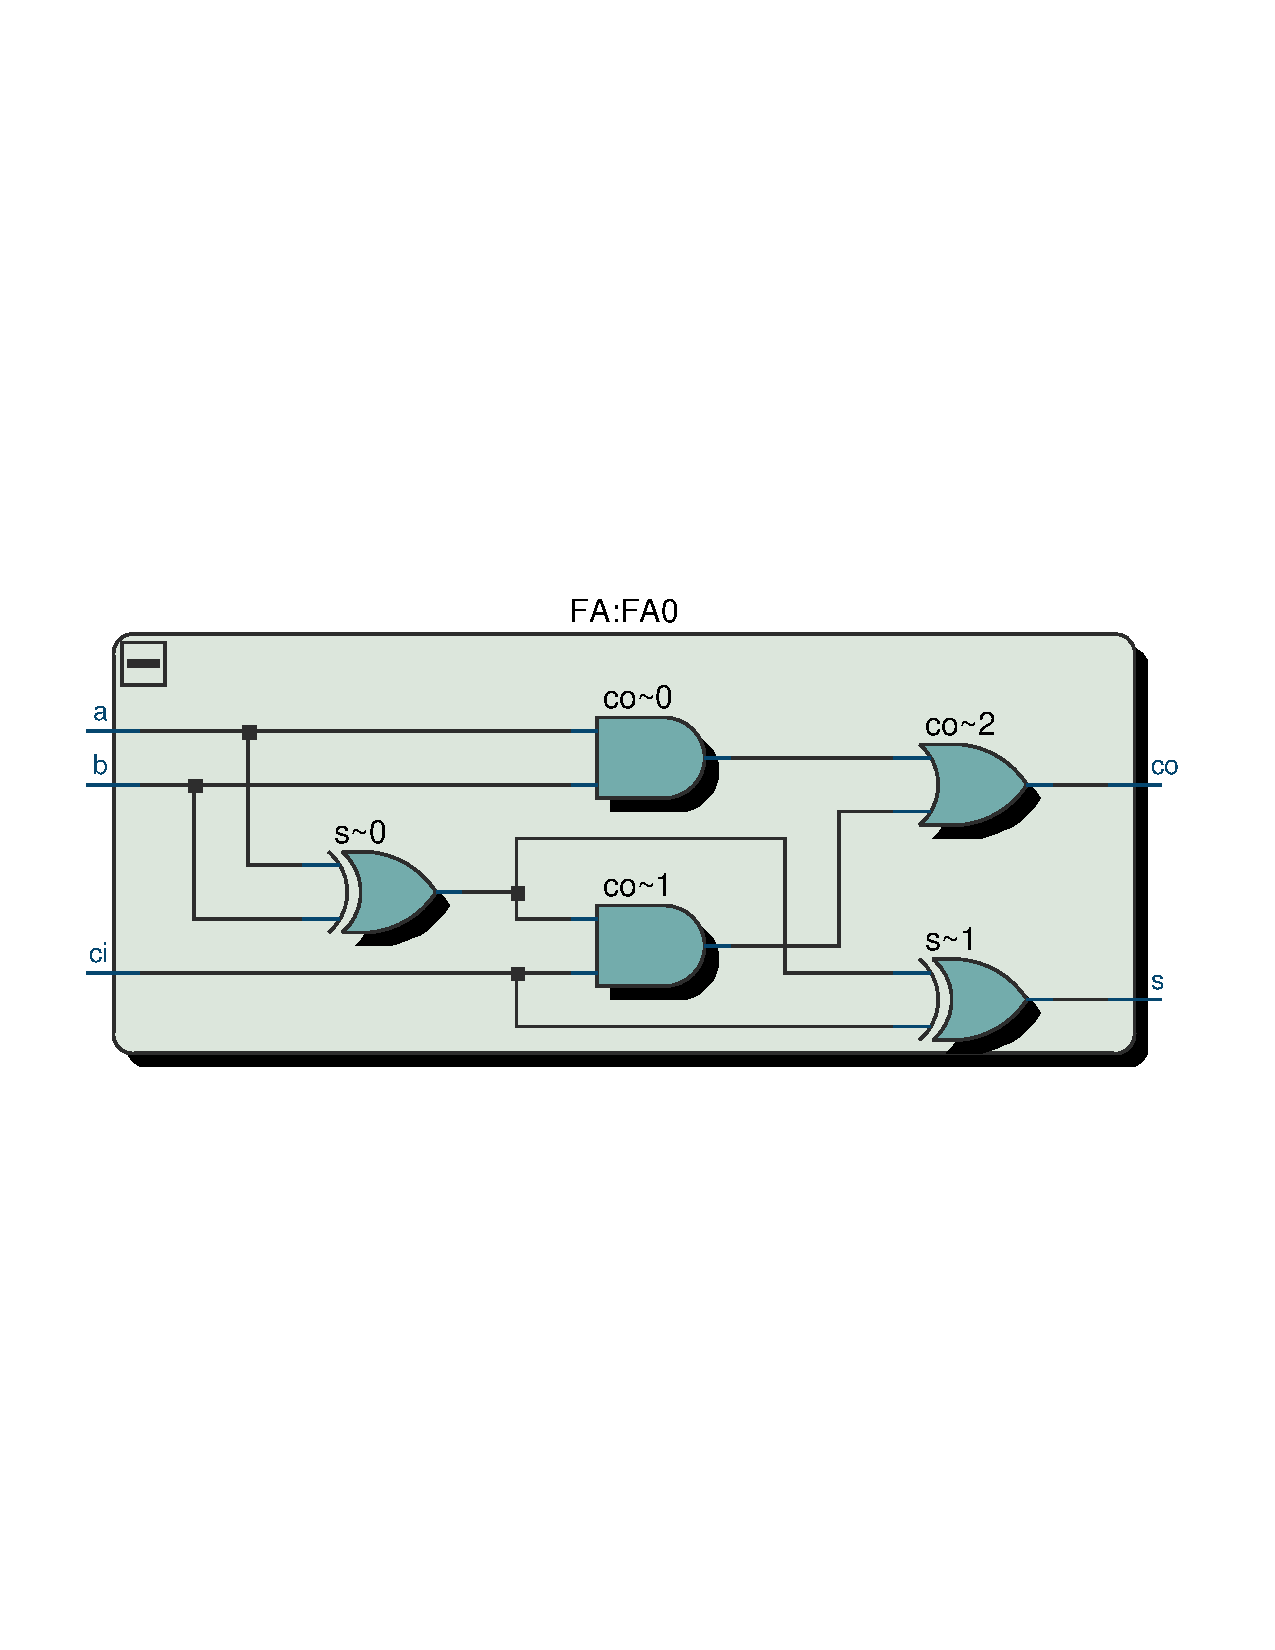
\includegraphics[scale=0.6, clip, trim={0cm 10cm 0cm 10.6cm}]{images/Exc1_FA_RTL.pdf}
\caption*{Full adder}
\end{figure}

\begin{figure}[H]
\centering
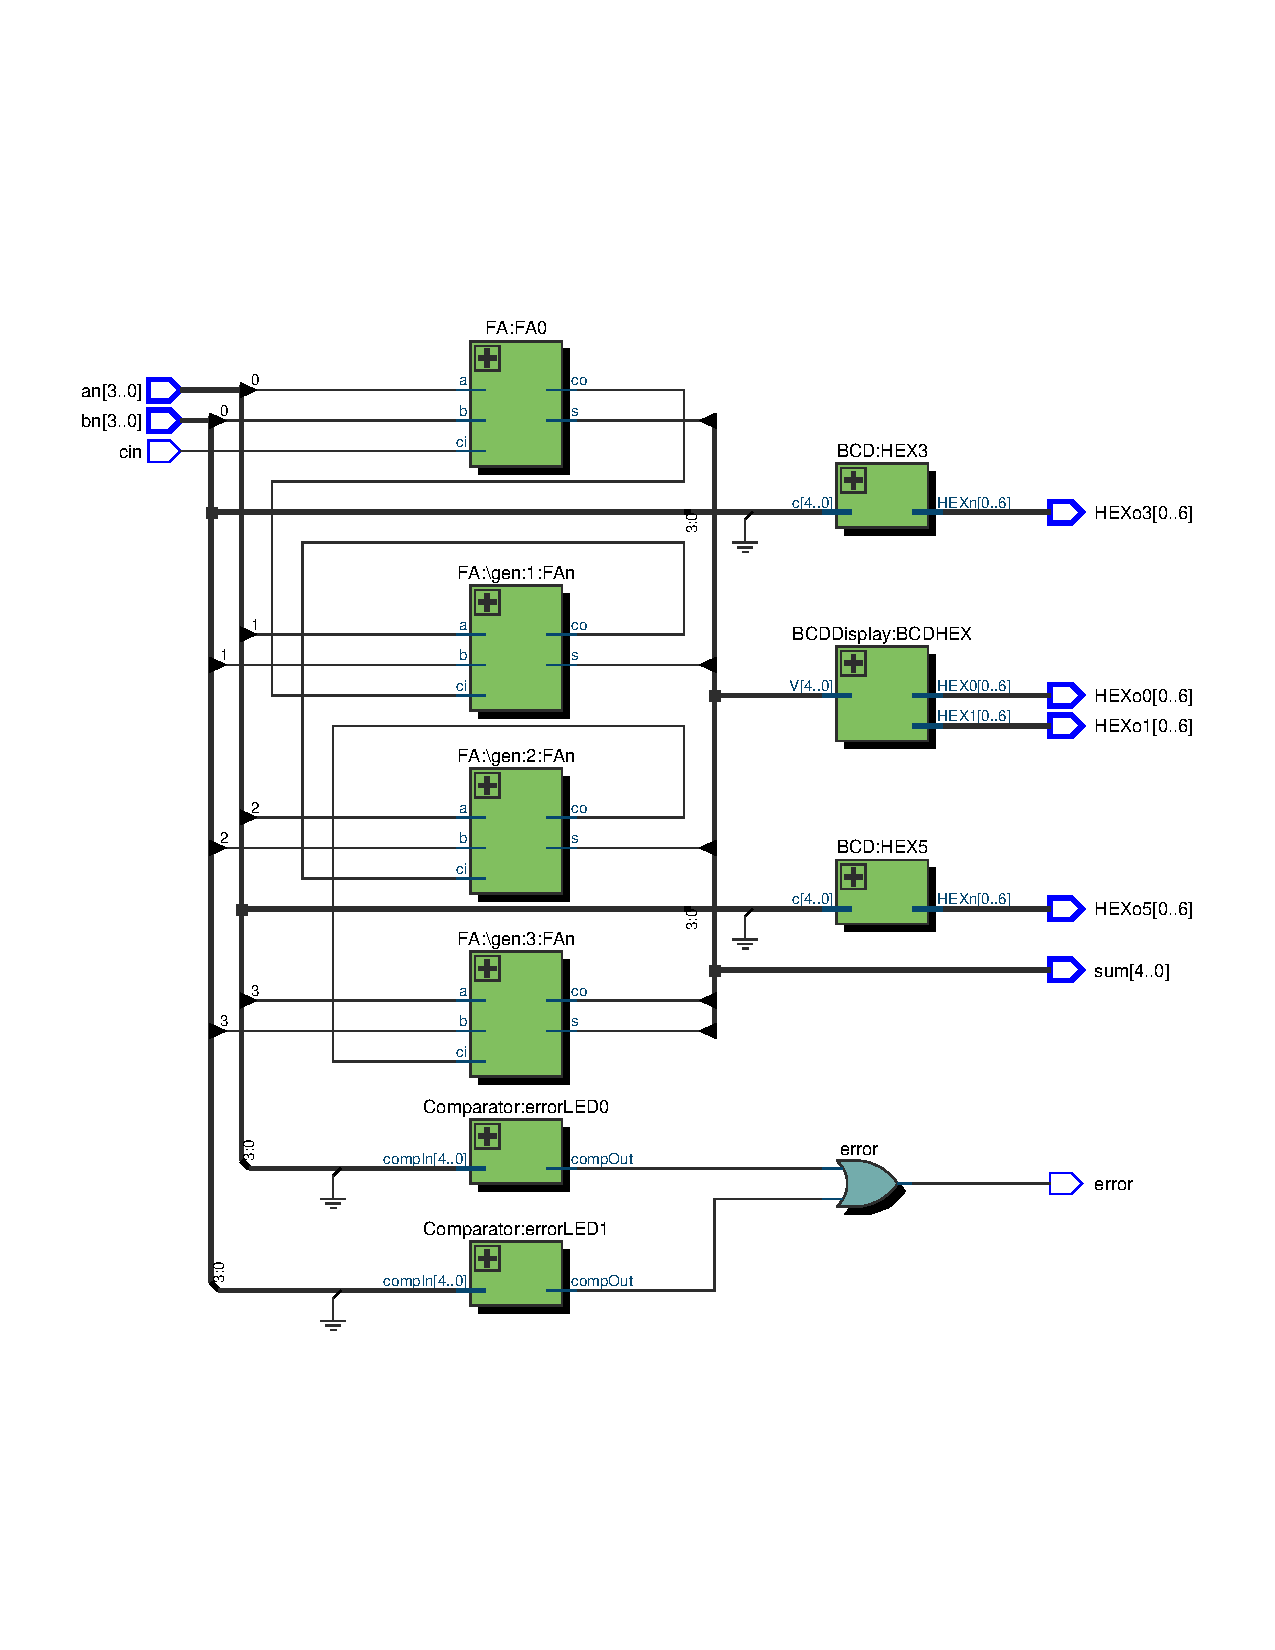
\includegraphics[scale=0.7, clip, trim={0cm 5cm 0cm 5cm}]{images/Exc2_RTL.pdf}
\caption*{Top level}
\end{figure}

\newpage
\section{Known how to program BCD adder}
\subsection{Code}

\subsubsection{BCD.vhd}
\begin{minted}{vhdl}
LIBRARY ieee;
USE ieee.std_logic_1164.ALL;

ENTITY BCD IS
	PORT (
		c : IN STD_LOGIC_VECTOR(4 DOWNTO 0);
		HEXn : OUT STD_LOGIC_VECTOR(0 TO 6)
	);
END BCD;

ARCHITECTURE behavior OF BCD IS
	SIGNAL HEX : STD_LOGIC_VECTOR(0 TO 6);
BEGIN
	HEXn <= NOT(HEX);
	WITH c SELECT
		HEX <= "1111110" WHEN "00000",
		"0110000" WHEN "00001",
		"1101101" WHEN "00010",
		"1111001" WHEN "00011",
		"0110011" WHEN "00100",
		"1011011" WHEN "00101",
		"1011111" WHEN "00110",
		"1110000" WHEN "00111",
		"1111111" WHEN "01000",
		"1111011" WHEN "01001",
		"0000000" WHEN OTHERS;
END behavior;
\end{minted}

\subsubsection{Exc3.vhd}
\begin{minted}{vhdl}
LIBRARY ieee;
USE ieee.std_logic_1164.ALL;
USE ieee.numeric_std.ALL;

ENTITY Exc3 IS
	PORT (
		an : IN STD_LOGIC_VECTOR(3 DOWNTO 0);
		bn : IN STD_LOGIC_VECTOR(3 DOWNTO 0);
		cin : IN STD_LOGIC_VECTOR(0 DOWNTO 0);
		HEXo0 : OUT STD_LOGIC_VECTOR(0 TO 6);
		HEXo1 : OUT STD_LOGIC_VECTOR(0 TO 6);
		HEXo3 : OUT STD_LOGIC_VECTOR(0 TO 6);
		HEXo5 : OUT STD_LOGIC_VECTOR(0 TO 6);
		sum : OUT STD_LOGIC_VECTOR(4 DOWNTO 0);
		error : OUT STD_LOGIC
	);
END ENTITY;

ARCHITECTURE arch OF Exc3 IS
	SIGNAL sn : STD_LOGIC_VECTOR(4 DOWNTO 0);
	SIGNAL digit1, digit0 : STD_LOGIC_VECTOR(4 DOWNTO 0);

	COMPONENT BCD IS
		PORT (
			c : IN STD_LOGIC_VECTOR(4 DOWNTO 0);
			HEXn : OUT STD_LOGIC_VECTOR(0 TO 6)
		);
	END COMPONENT;
BEGIN
	HEX5 : BCD PORT MAP(c => '0' & an, HEXn => HEXo5);
	HEX3 : BCD PORT MAP(c => '0' & bn, HEXn => HEXo3);

	sn <= STD_LOGIC_VECTOR(unsigned('0' & an) + unsigned('0' & bn) + unsigned(cin));
	digit1 <= STD_LOGIC_VECTOR(unsigned(sn) / 10);
	digit0 <= STD_LOGIC_VECTOR(unsigned(sn) MOD 10);

	HEX01 : BCD PORT MAP(c => digit1, HEXn => HEXo1);
	HEX00 : BCD PORT MAP(c => digit0, HEXn => HEXo0);

	sum <= sn;

	error <= '1' WHEN (unsigned(an) > 9 OR unsigned(bn) > 9) ELSE '0';
END ARCHITECTURE;
\end{minted}

\subsection{Waveform}
\begin{figure}[H]
\centering
\includegraphics[scale=0.7]{images/Exc2_waveform.png}
\end{figure}

\subsection{Result of RTL viewer}
\begin{figure}[H]
\centering
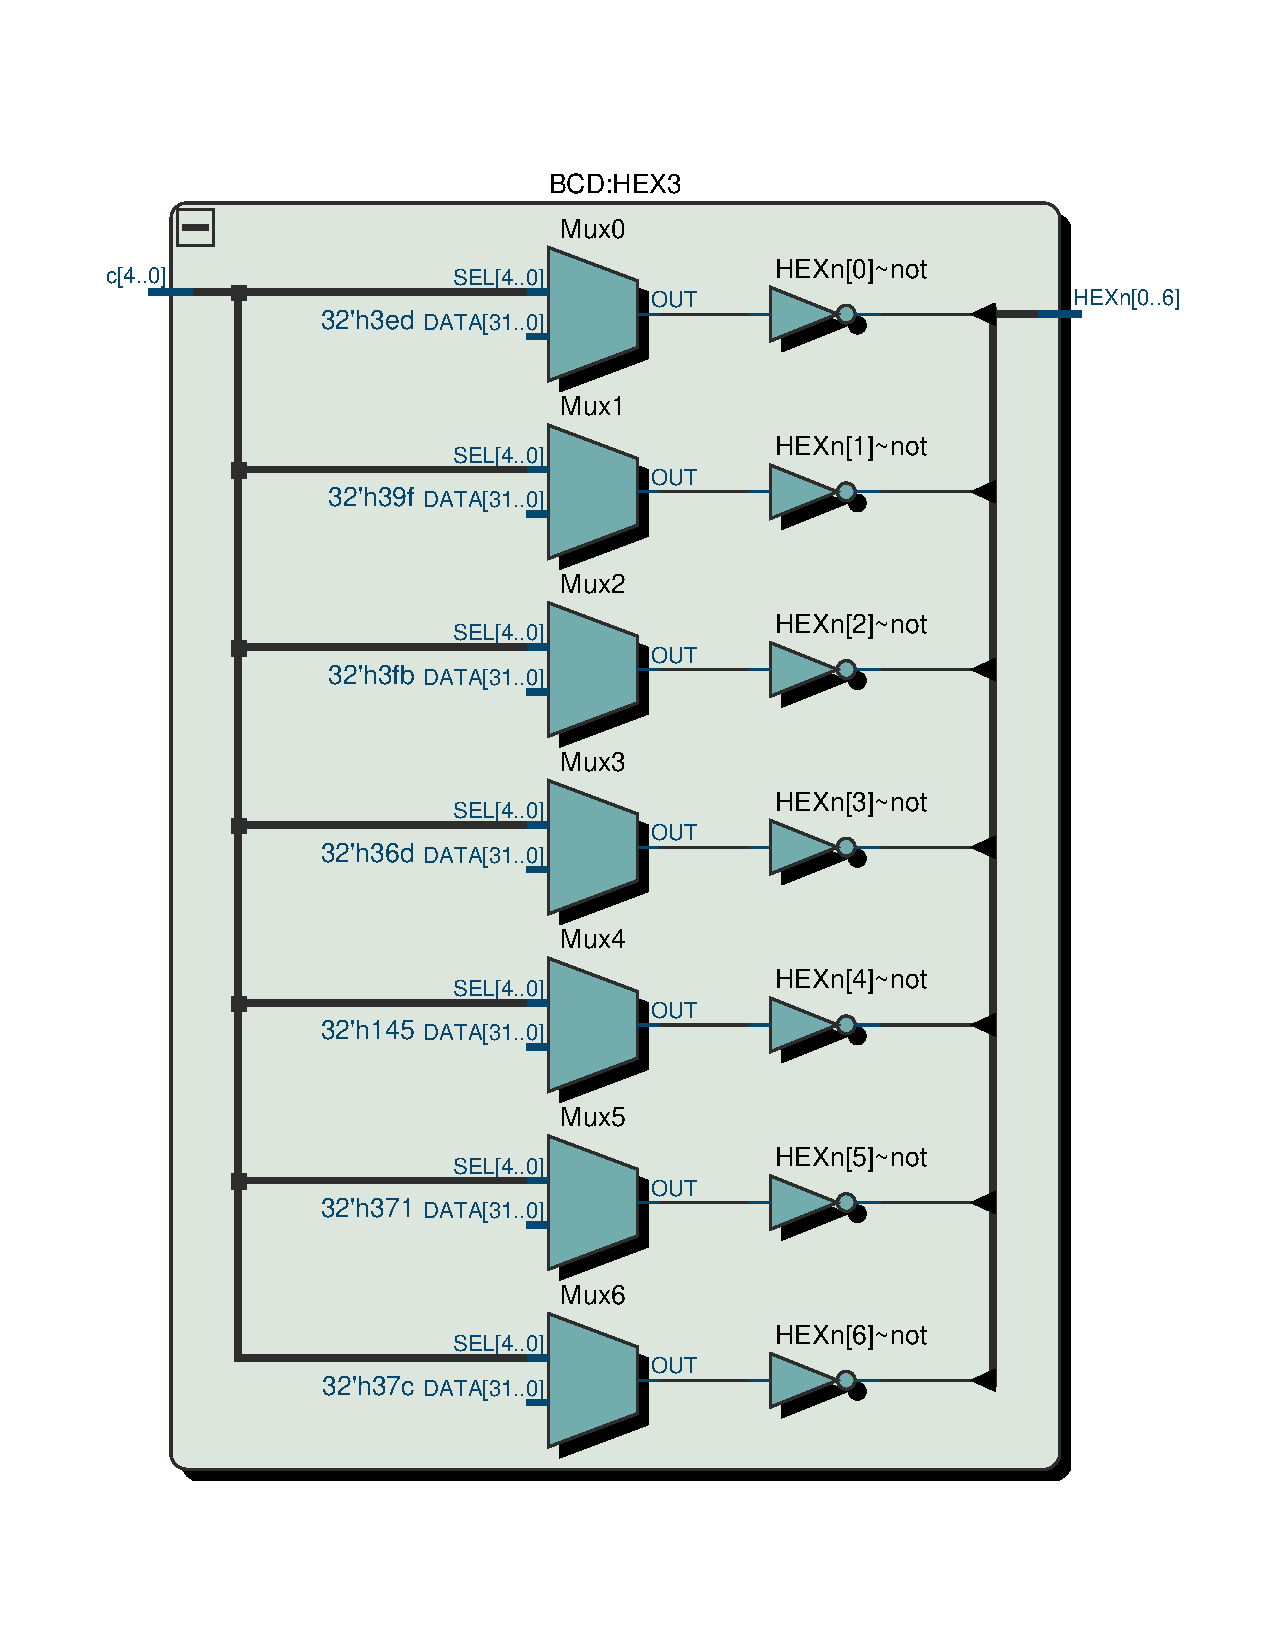
\includegraphics[scale=0.5, clip, trim={0cm 3cm 0cm 3.3cm}]{images/Exc2_BCD_RTL.pdf}
\caption*{BCD MUX}
\end{figure}

\begin{figure}[H]
\centering
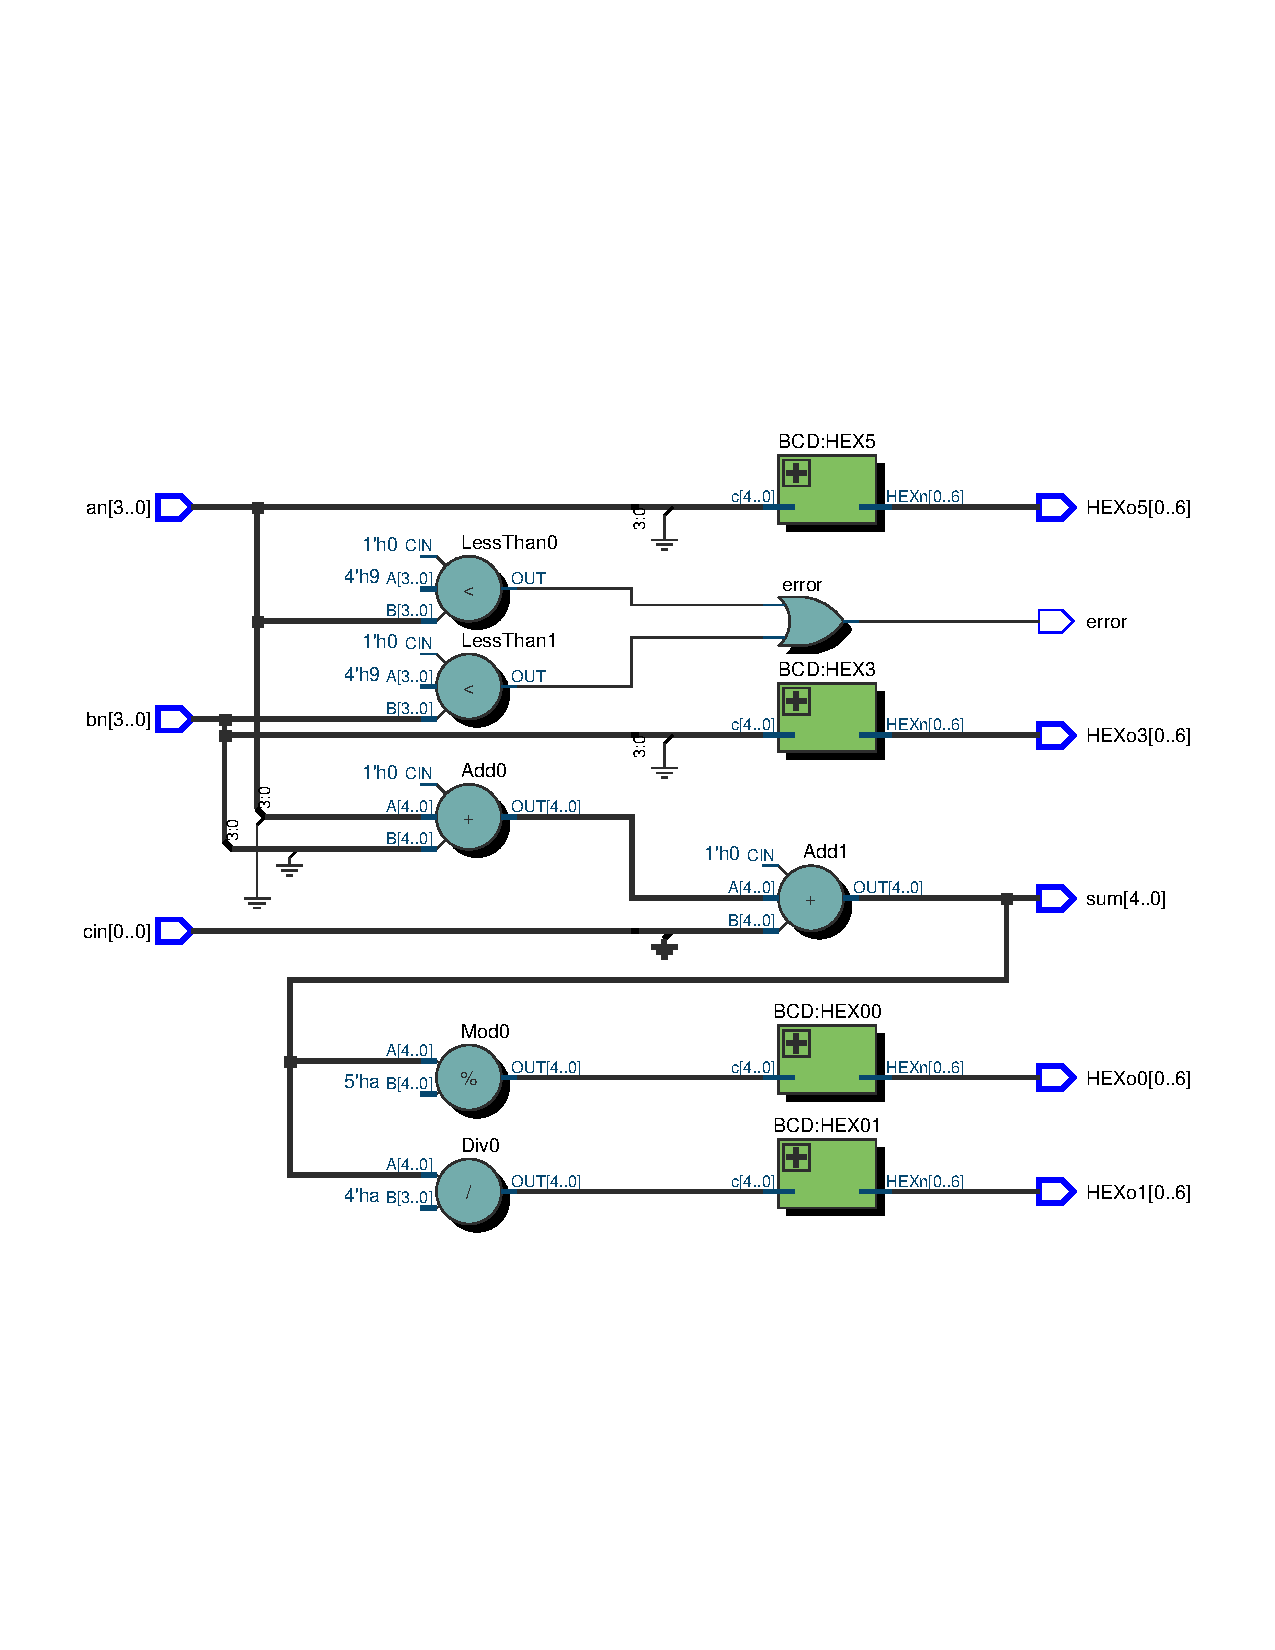
\includegraphics[scale=0.7, clip, trim={0cm 7cm 0cm 7cm}]{images/Exc3_RTL.pdf}
\caption*{Top level}
\end{figure}

The circuit is simplier when relying more on the VHDL compiler.

\section{Known how to program a master-slave D flip-flop}

\subsection{Code}
\subsubsection{DFFn.vhd}
\begin{minted}{vhdl}
LIBRARY ieee;
USE ieee.std_logic_1164.ALL;

ENTITY DFFn IS
	PORT (
		DClk, Din : IN STD_LOGIC;
		DQ : OUT STD_LOGIC
	);
END DFFn;

ARCHITECTURE Structural OF DFFn IS
	SIGNAL R_g, S_g, Qa, Qb, S, R : STD_LOGIC;
	ATTRIBUTE KEEP : BOOLEAN;
	ATTRIBUTE KEEP OF R_g, S_g, Qa, Qb : SIGNAL IS TRUE;

BEGIN
	S <= Din;
	R <= NOT(Din);
	R_g <= R AND DClk;
	S_g <= S AND DClk;
	Qa <= R_g NOR Qb;
	Qb <= S_g NOR Qa;
	DQ <= Qa;
END Structural;
\end{minted}

\subsubsection{Exc4.vhd}
\begin{minted}{vhdl}
LIBRARY ieee;
USE ieee.std_logic_1164.ALL;

ENTITY Exc4 IS
	PORT (
		D, Clk : IN STD_LOGIC;
		Q : OUT STD_LOGIC
	);
END Exc4;

ARCHITECTURE arch OF Exc4 IS
	SIGNAL Qm : STD_LOGIC;
	COMPONENT DFFn IS
		PORT (
			DClk, Din : IN STD_LOGIC;
			DQ : OUT STD_LOGIC
		);
	END COMPONENT;
BEGIN
	DFF1 : DFFn PORT MAP(DClk => NOT(Clk), Din => D, DQ => Qm);
	DFF0 : DFFn PORT MAP(DClk => Clk, Din => Qm, DQ => Q);
END ARCHITECTURE;
\end{minted}

\subsection{Waveform}
\begin{figure}[H]
\centering
\includegraphics[scale=0.7]{images/Exc4_waveform.png}
\end{figure}

\subsection{Result of RTL viewer}
\begin{figure}[H]
\centering
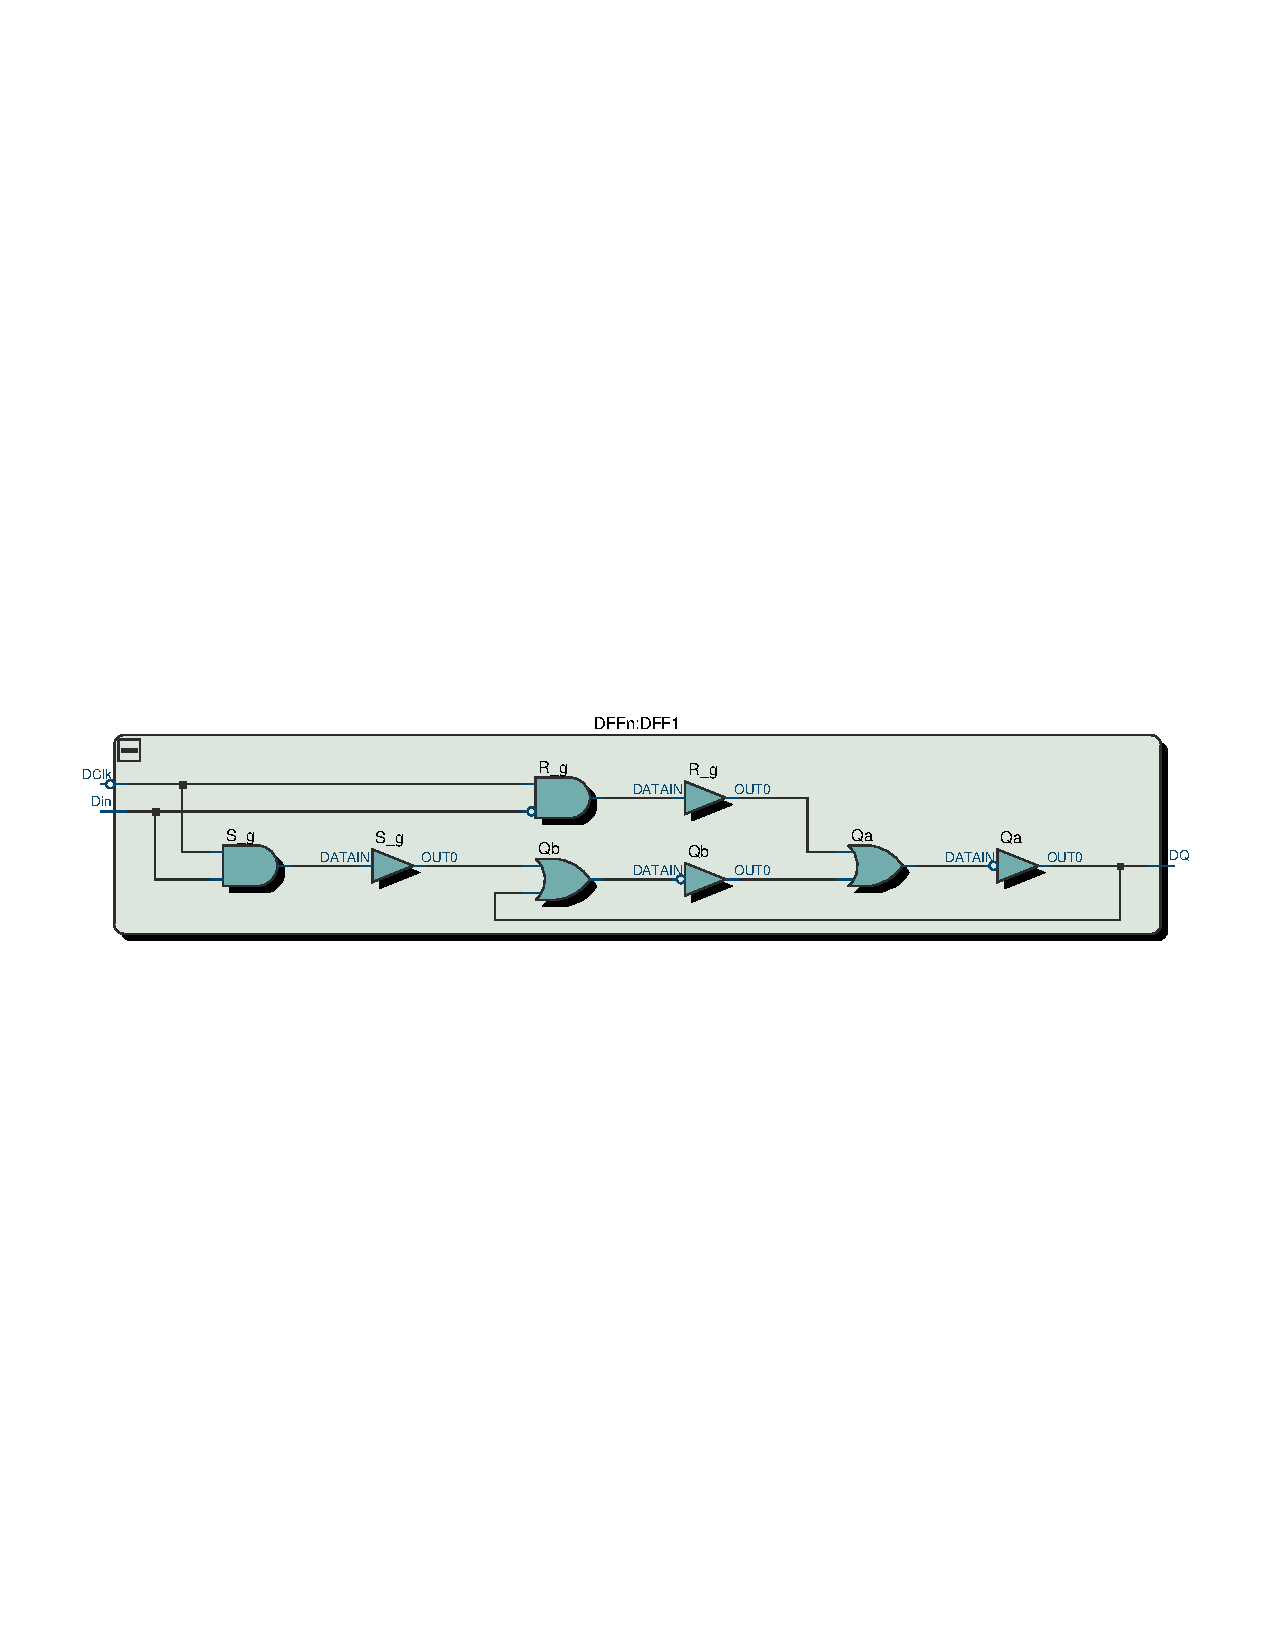
\includegraphics[scale=0.7, clip, trim={0cm 12cm 0cm 12.4cm}]{images/Exc4_DFF_RTL.pdf}
\caption*{D flip-flop}
\end{figure}

\begin{figure}[H]
\centering
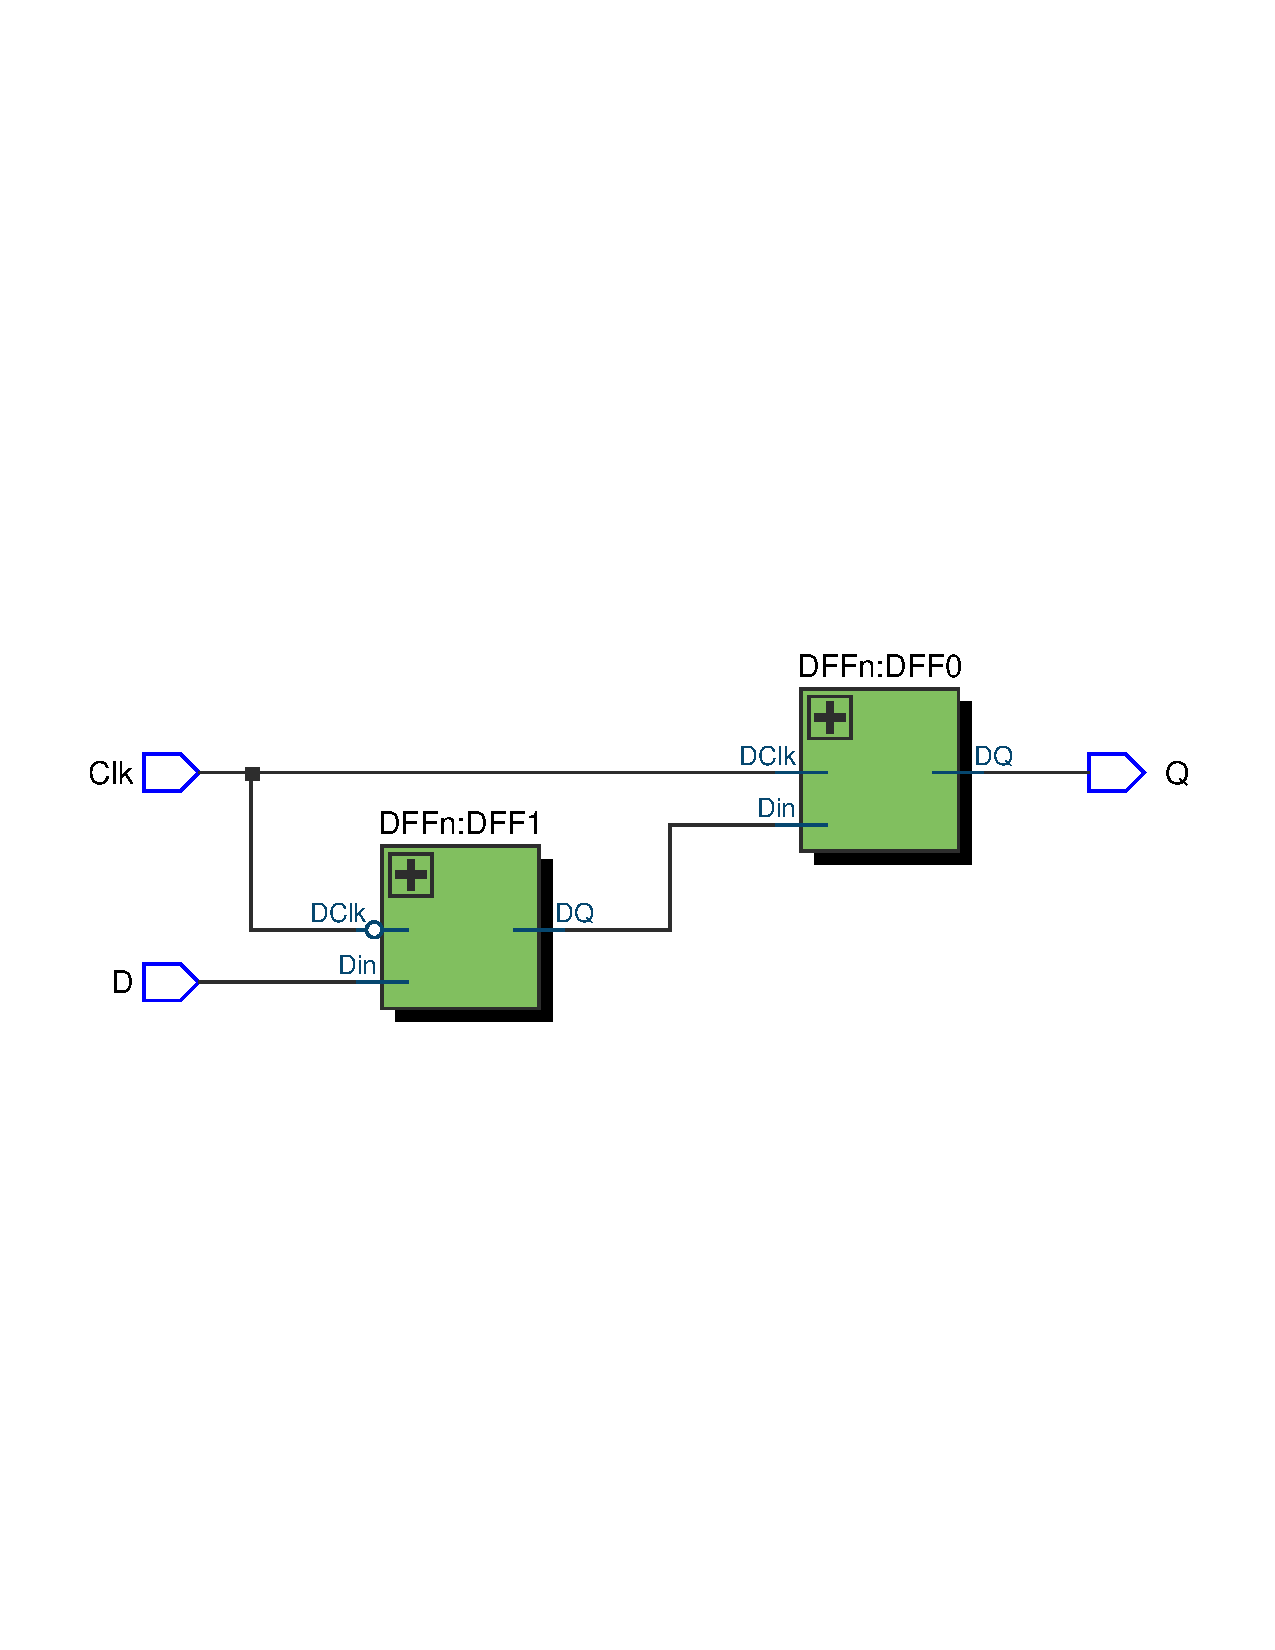
\includegraphics[scale=0.6, clip, trim={0cm 10cm 0cm 11cm}]{images/Exc4_RTL.pdf}
\caption*{Top level}
\end{figure}

\section{Known how to program a master-slave D flip-flopCompare the different behavior of the three storage elements: a gated D latch, a positive-edge triggered D flip-flop, and a negative-edge triggered D flip-flop.}

\subsection{Code}
\subsubsection{DL.vhd}
\begin{minted}{vhdl}
LIBRARY ieee;
USE ieee.std_logic_1164.ALL;
ENTITY DL IS
	PORT (
		DLin, DLClk : IN STD_LOGIC;
		DLQ : OUT STD_LOGIC);
END DL;
ARCHITECTURE Behavior OF DL IS
BEGIN
	PROCESS (DLin, DLClk)
	BEGIN
		IF DLClk = '1' THEN
			DLQ <= DLin;
		END IF;
	END PROCESS;
END Behavior;
\end{minted}

\subsubsection{DFFn.vhd}
\begin{minted}{vhdl}
LIBRARY ieee;
USE ieee.std_logic_1164.ALL;

ENTITY DFFn IS
	PORT (
		DClk, Din : IN STD_LOGIC;
		DQ : OUT STD_LOGIC
	);
END DFFn;

ARCHITECTURE Structural OF DFFn IS
BEGIN
	PROCESS (DClk)
	BEGIN
		IF rising_edge(DClk) THEN
			DQ <= Din;
		END IF;
	END PROCESS;
END Structural;
\end{minted}

\subsubsection{Exc5.vhd}
\begin{minted}{vhdl}
LIBRARY ieee;
USE ieee.std_logic_1164.ALL;
USE ieee.numeric_std.ALL;

ENTITY Exc5 IS
	PORT (
		D, Clk : IN STD_LOGIC;
		Qa, Qb, Qc : OUT STD_LOGIC
	);
END Exc5;

ARCHITECTURE arch OF Exc5 IS
	COMPONENT DL IS
		PORT (
			DLin, DLClk : IN STD_LOGIC;
			DLQ : OUT STD_LOGIC);
	END COMPONENT;

	COMPONENT DFFn IS
		PORT (
			Din, DClk : IN STD_LOGIC;
			DQ : OUT STD_LOGIC);
	END COMPONENT;
BEGIN
	DFF2 : DL PORT MAP(DLin => D, DLClk => Clk, DLQ => Qa);
	DFF1 : DFFn PORT MAP(Din => D, DClk => Clk, DQ => Qb);
	DFF0 : DFFn PORT MAP(Din => D, DClk => NOT(Clk), DQ => Qc);
END ARCHITECTURE;
\end{minted}

\subsection{Waveform}
\begin{figure}[H]
\centering
\includegraphics[scale=0.8]{images/Exc5_waveform.png}
\end{figure}

\subsection{Result of RTL viewer}
\begin{figure}[H]
\centering
\subfloat[][D latch]{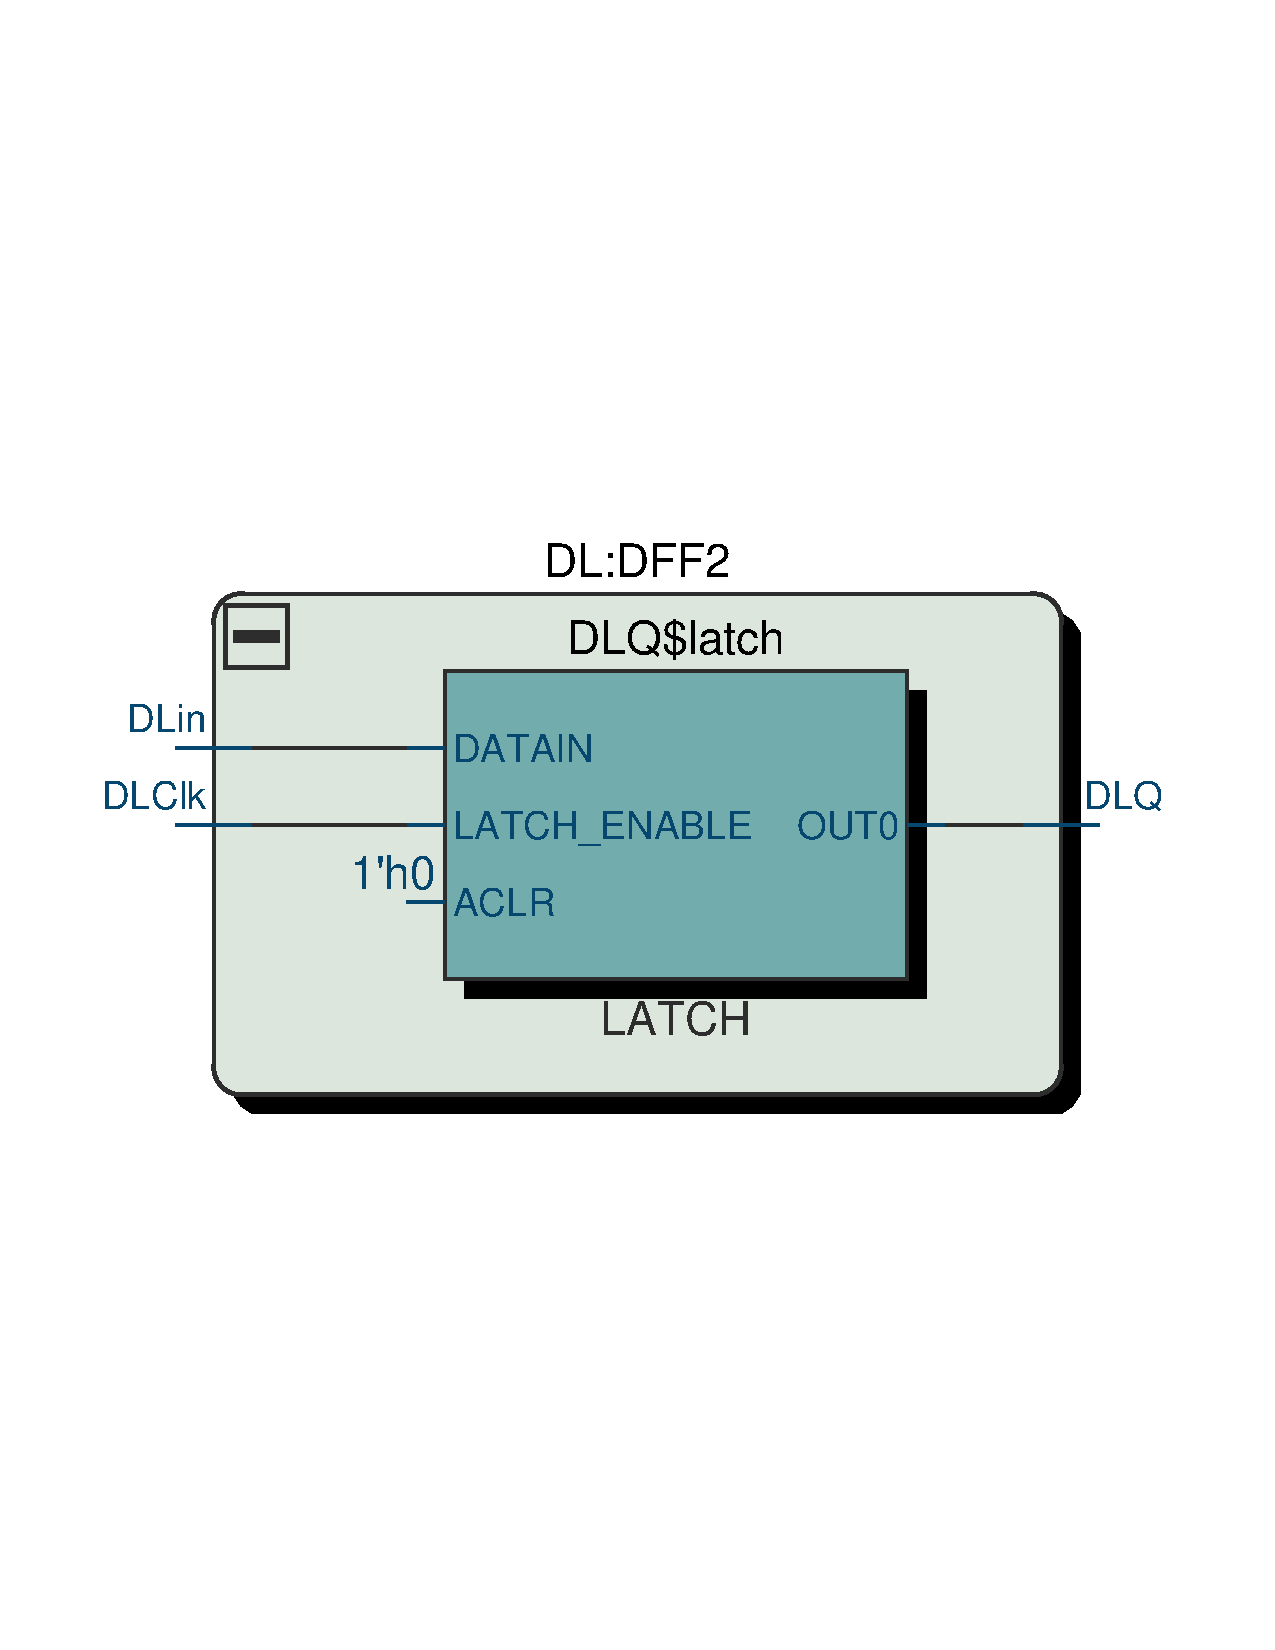
\includegraphics[scale=0.4, clip, trim={0cm 8cm 0cm 10cm}]{images/Exc5_DLatch_RTL.pdf}}
\subfloat[][D flip-flop]{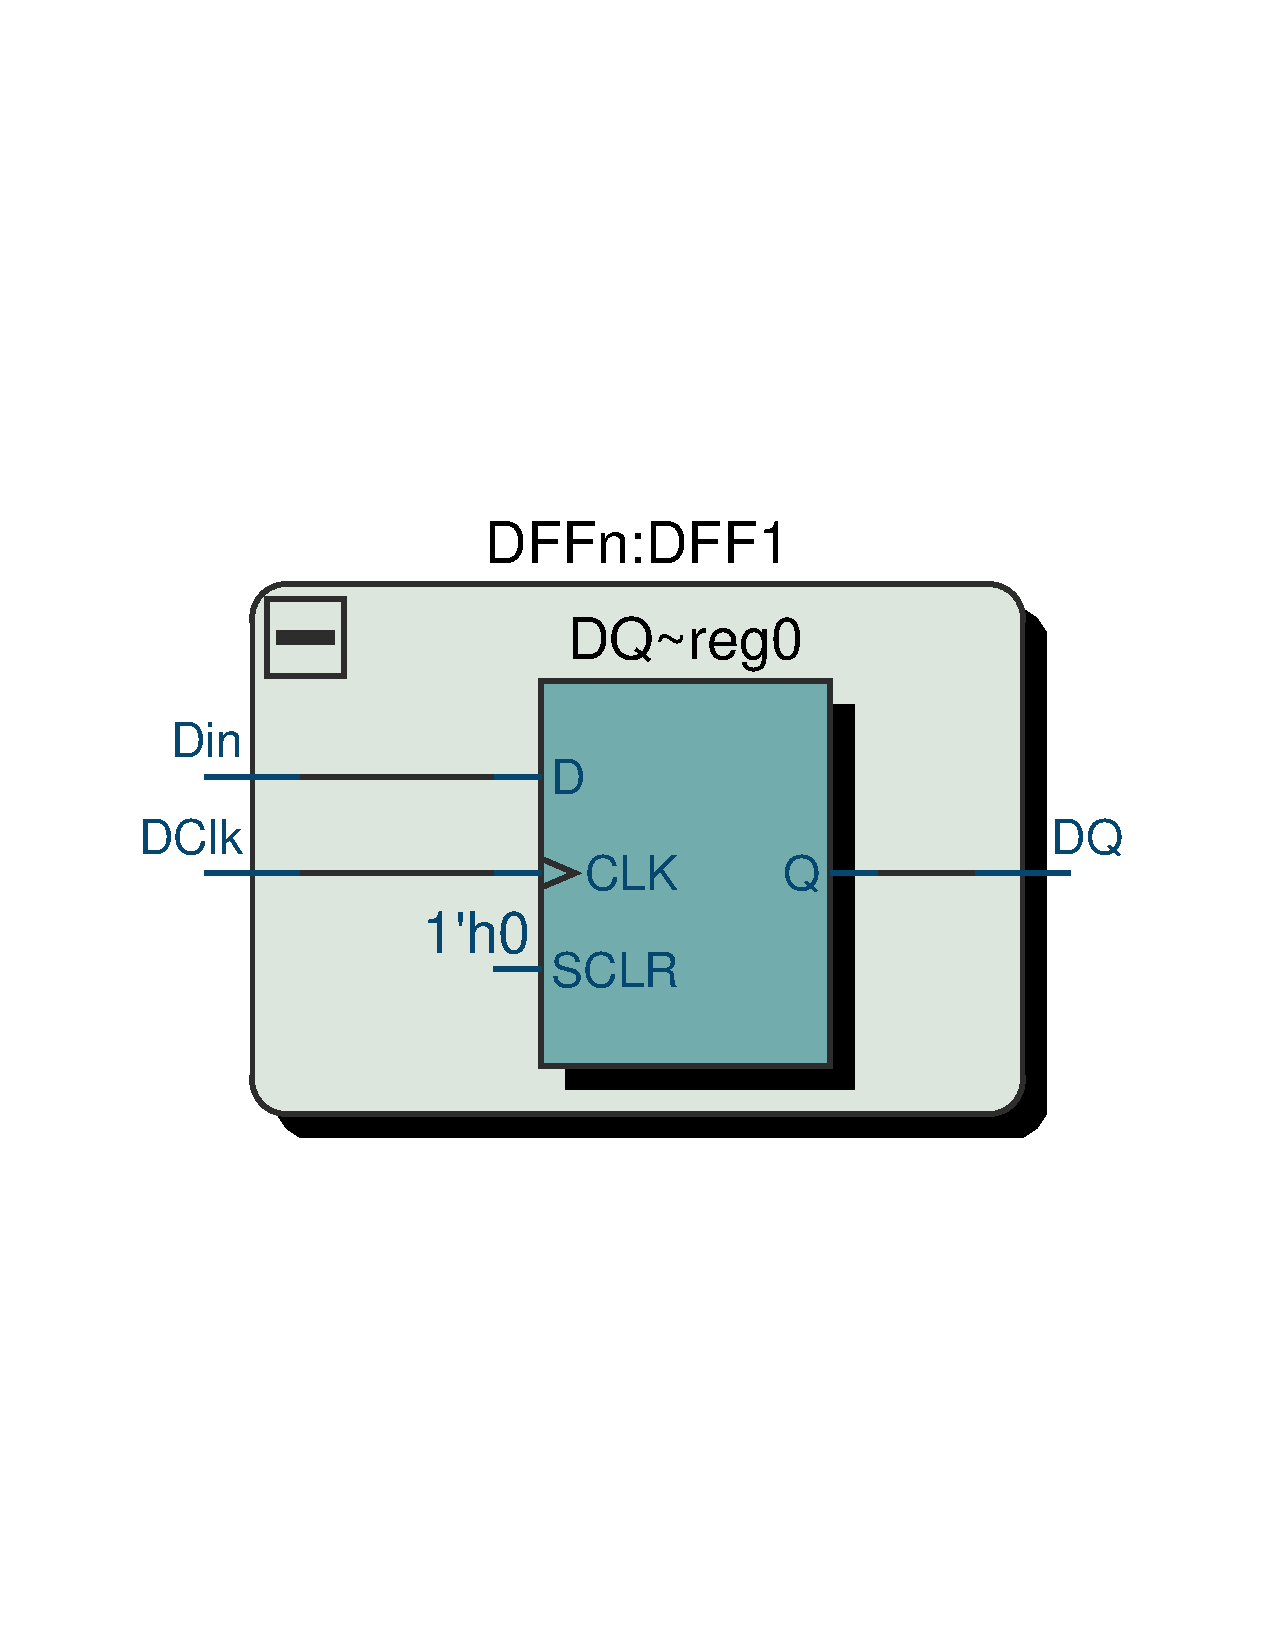
\includegraphics[scale=0.4, clip, trim={0cm 8cm 0cm 9.8cm}]{images/Exc5_DFF_RTL.pdf}}
\end{figure}

\begin{figure}[H]
\centering
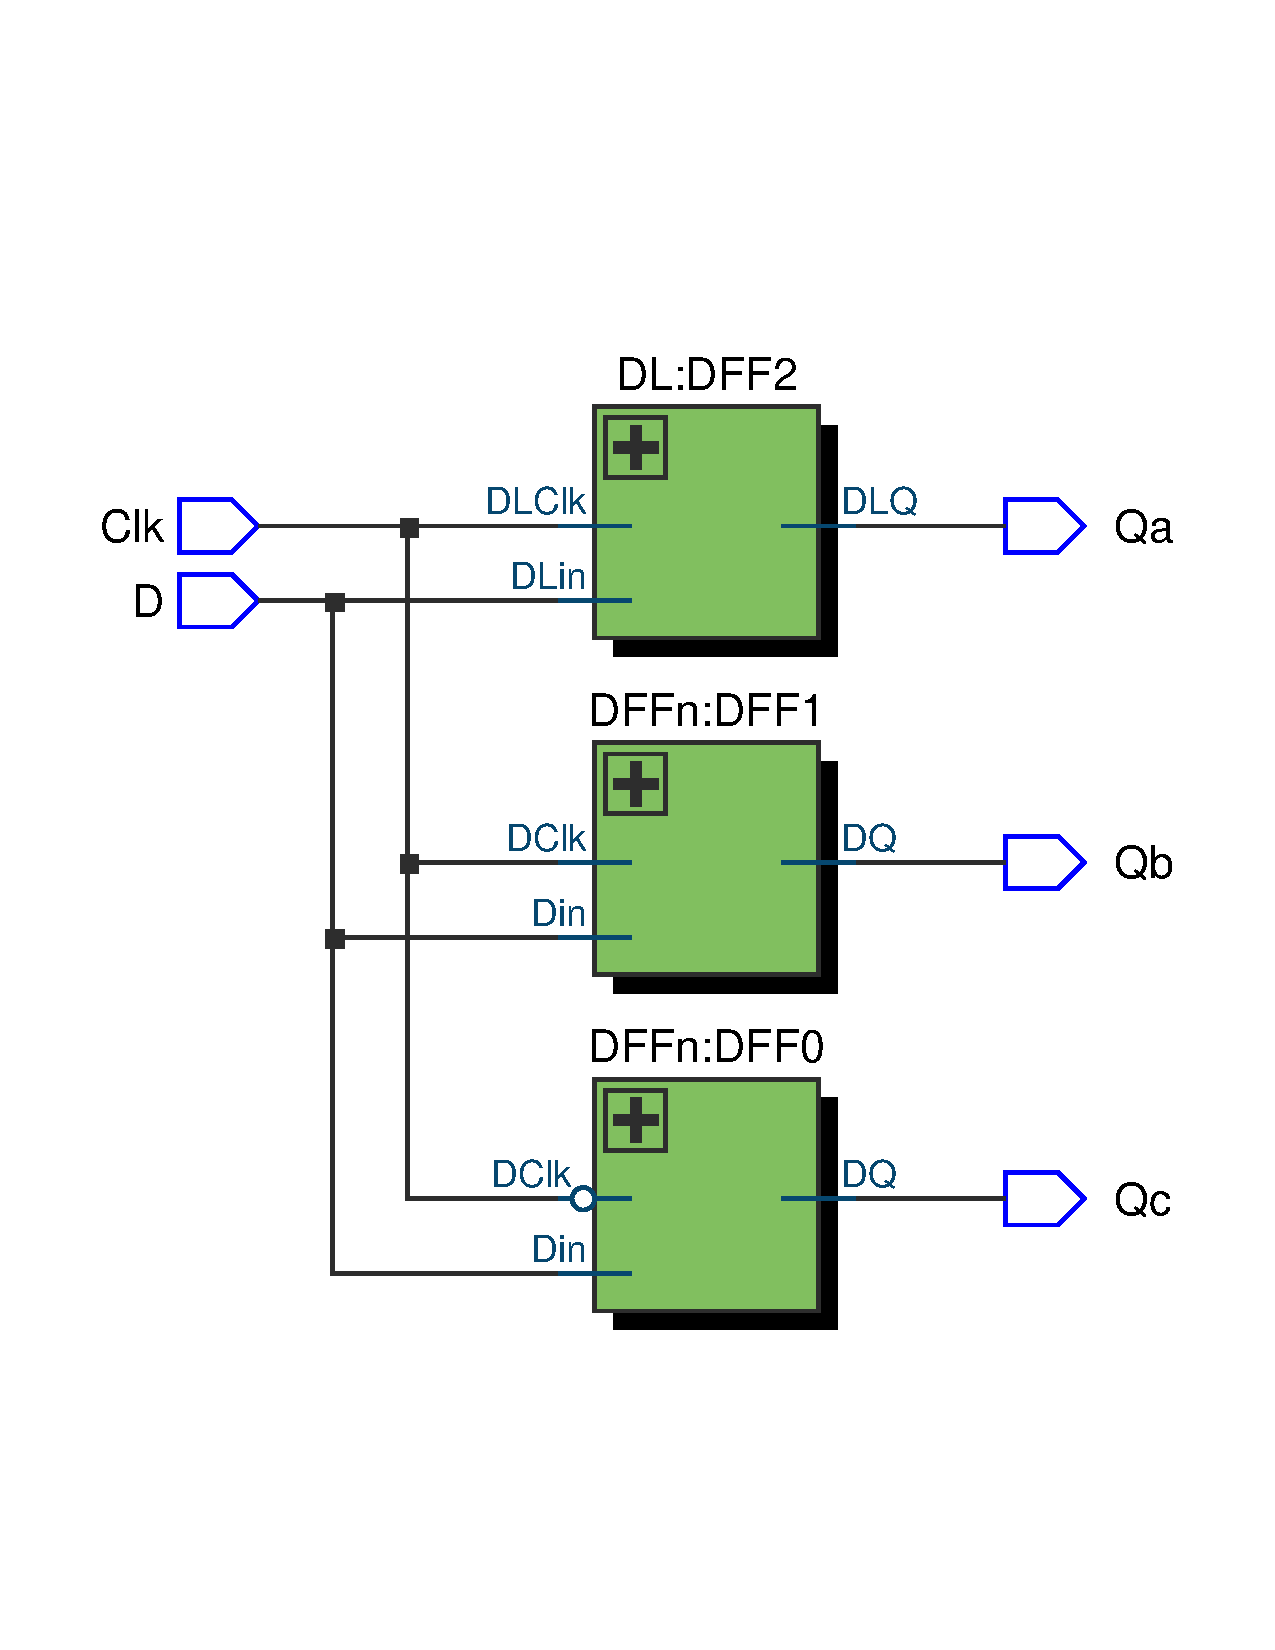
\includegraphics[scale=0.4, clip, trim={0cm 5cm 0cm 5cm}]{images/Exc5_RTL.pdf}
\caption*{Top level}
\end{figure}

\section{Apply all the previous experiments}

\subsection{Code}
\subsubsection{DFFn.vhd}
\begin{minted}{vhdl}
LIBRARY ieee;
USE ieee.std_logic_1164.ALL;
ENTITY DFFn IS
	PORT (
		Din, DClk, Drst : IN STD_LOGIC;
		DQ : OUT STD_LOGIC);
END DFFn;
ARCHITECTURE Behavior OF DFFn IS
BEGIN
	PROCESS (Drst, DClk)
	BEGIN
		IF rising_edge(DClk) THEN
			DQ <= Din;
		END IF;
		IF Drst = '1' THEN
			DQ <= '0';
		END IF;
	END PROCESS;
END Behavior;
\end{minted}

\subsubsection{EightBitReg.vhd}
\begin{minted}{vhdl}
LIBRARY ieee;
USE ieee.std_logic_1164.ALL;
USE ieee.numeric_std.ALL;

ENTITY EightBitReg IS
	PORT (
		EBRClk, EBRrst : IN STD_LOGIC;
		EBRD : IN STD_LOGIC_VECTOR(7 DOWNTO 0);
		EBRQ : OUT STD_LOGIC_VECTOR(7 DOWNTO 0)
	);
END EightBitReg;

ARCHITECTURE arch OF EightBitReg IS
	COMPONENT DFFn IS
		PORT (
			Din, DClk, Drst : IN STD_LOGIC;
			DQ : OUT STD_LOGIC);
	END COMPONENT;
BEGIN
	gen : FOR i IN 7 DOWNTO 0 GENERATE
		DFFs : DFFn PORT MAP(Din => EBRD(i), DClk => EBRClk, Drst => EBRrst, DQ => EBRQ(i));
	END GENERATE;
END ARCHITECTURE;
\end{minted}

\subsubsection{HEXDisplay.vhd}
\begin{minted}{vhdl}
LIBRARY ieee;
USE ieee.std_logic_1164.ALL;

ENTITY HEXDisplay IS
	PORT (
		c : IN STD_LOGIC_VECTOR(3 DOWNTO 0);
		HEXn : OUT STD_LOGIC_VECTOR(0 TO 6)
	);
END HEXDisplay;

ARCHITECTURE behavior OF HEXDisplay IS
	SIGNAL HEX : STD_LOGIC_VECTOR(0 TO 6);
BEGIN
	HEXn <= NOT(HEX);
	WITH c SELECT
		HEX <= "1111110" WHEN "0000",
		"0110000" WHEN "0001",
		"1101101" WHEN "0010",
		"1111001" WHEN "0011",
		"0110011" WHEN "0100",
		"1011011" WHEN "0101",
		"1011111" WHEN "0110",
		"1110000" WHEN "0111",
		"1111111" WHEN "1000",
		"1111011" WHEN "1001",

		"1110111" WHEN "1010",
		"0011111" WHEN "1011",
		"1001110" WHEN "1100",
		"0111101" WHEN "1101",
		"1001111" WHEN "1110",
		"1000111" WHEN "1111",
		"0000000" WHEN OTHERS;
END behavior; -- behavior
\end{minted}

\subsubsection{Exc6.vhd}
\begin{minted}{vhdl}
LIBRARY ieee;
USE ieee.std_logic_1164.ALL;
USE ieee.numeric_std.ALL;

ENTITY Exc6 IS
	PORT (
		ClkN, rstN : IN STD_LOGIC;
		D : IN STD_LOGIC_VECTOR(7 DOWNTO 0);
		cout : OUT STD_LOGIC;
		HEX5 : OUT STD_LOGIC_VECTOR(0 TO 6);
		HEX4 : OUT STD_LOGIC_VECTOR(0 TO 6);
		HEX3 : OUT STD_LOGIC_VECTOR(0 TO 6);
		HEX2 : OUT STD_LOGIC_VECTOR(0 TO 6);
		HEX1 : OUT STD_LOGIC_VECTOR(0 TO 6);
		HEX0 : OUT STD_LOGIC_VECTOR(0 TO 6)
	);
END Exc6;

ARCHITECTURE arch OF Exc6 IS
	SIGNAL sum : STD_LOGIC_VECTOR(8 DOWNTO 0);
	SIGNAL Q : STD_LOGIC_VECTOR(7 DOWNTO 0);
	SIGNAL Clk, rst : STD_LOGIC;
	COMPONENT EightBitReg IS
		PORT (
			EBRClk, EBRrst : IN STD_LOGIC;
			EBRD : IN STD_LOGIC_VECTOR(7 DOWNTO 0);
			EBRQ : OUT STD_LOGIC_VECTOR(7 DOWNTO 0)
		);
	END COMPONENT;

	COMPONENT HEXDisplay IS
		PORT (
			c : IN STD_LOGIC_VECTOR(3 DOWNTO 0);
			HEXn : OUT STD_LOGIC_VECTOR(0 TO 6)
		);
	END COMPONENT;
BEGIN
	Clk <= NOT(ClkN);
	rst <= NOT(rstN);
	sum <= STD_LOGIC_VECTOR(unsigned('0' & Q) + unsigned('0' & D));
	EBR : EightBitReg PORT MAP(EBRClk => Clk, EBRrst => rst, EBRD => D, EBRQ => Q);
	HEX05 : HEXDisplay PORT MAP(c => sum(7 DOWNTO 4), HEXn => HEX5);
	HEX04 : HEXDisplay PORT MAP(c => sum(3 DOWNTO 0), HEXn => HEX4);
	HEX03 : HEXDisplay PORT MAP(c => D(7 DOWNTO 4), HEXn => HEX3);
	HEX02 : HEXDisplay PORT MAP(c => D(3 DOWNTO 0), HEXn => HEX2);
	HEX01 : HEXDisplay PORT MAP(c => Q(7 DOWNTO 4), HEXn => HEX1);
	HEX00 : HEXDisplay PORT MAP(c => Q(3 DOWNTO 0), HEXn => HEX0);
	cout <= sum(8);
END ARCHITECTURE;
\end{minted}

\subsection{Waveform}
\begin{figure}[H]
\centering
\includegraphics[scale=0.65]{images/Exc6_waveform.png}
\end{figure}

\subsection{Result of RTL viewer}
\begin{figure}[H]
\centering
\subfloat[][D flip-flop]{\includegraphics[scale=0.3, clip, trim={2cm 8cm 2cm 9.1cm}]{images/Exc6_DFF_RTL.pdf}}
\subfloat[][8-bit register]{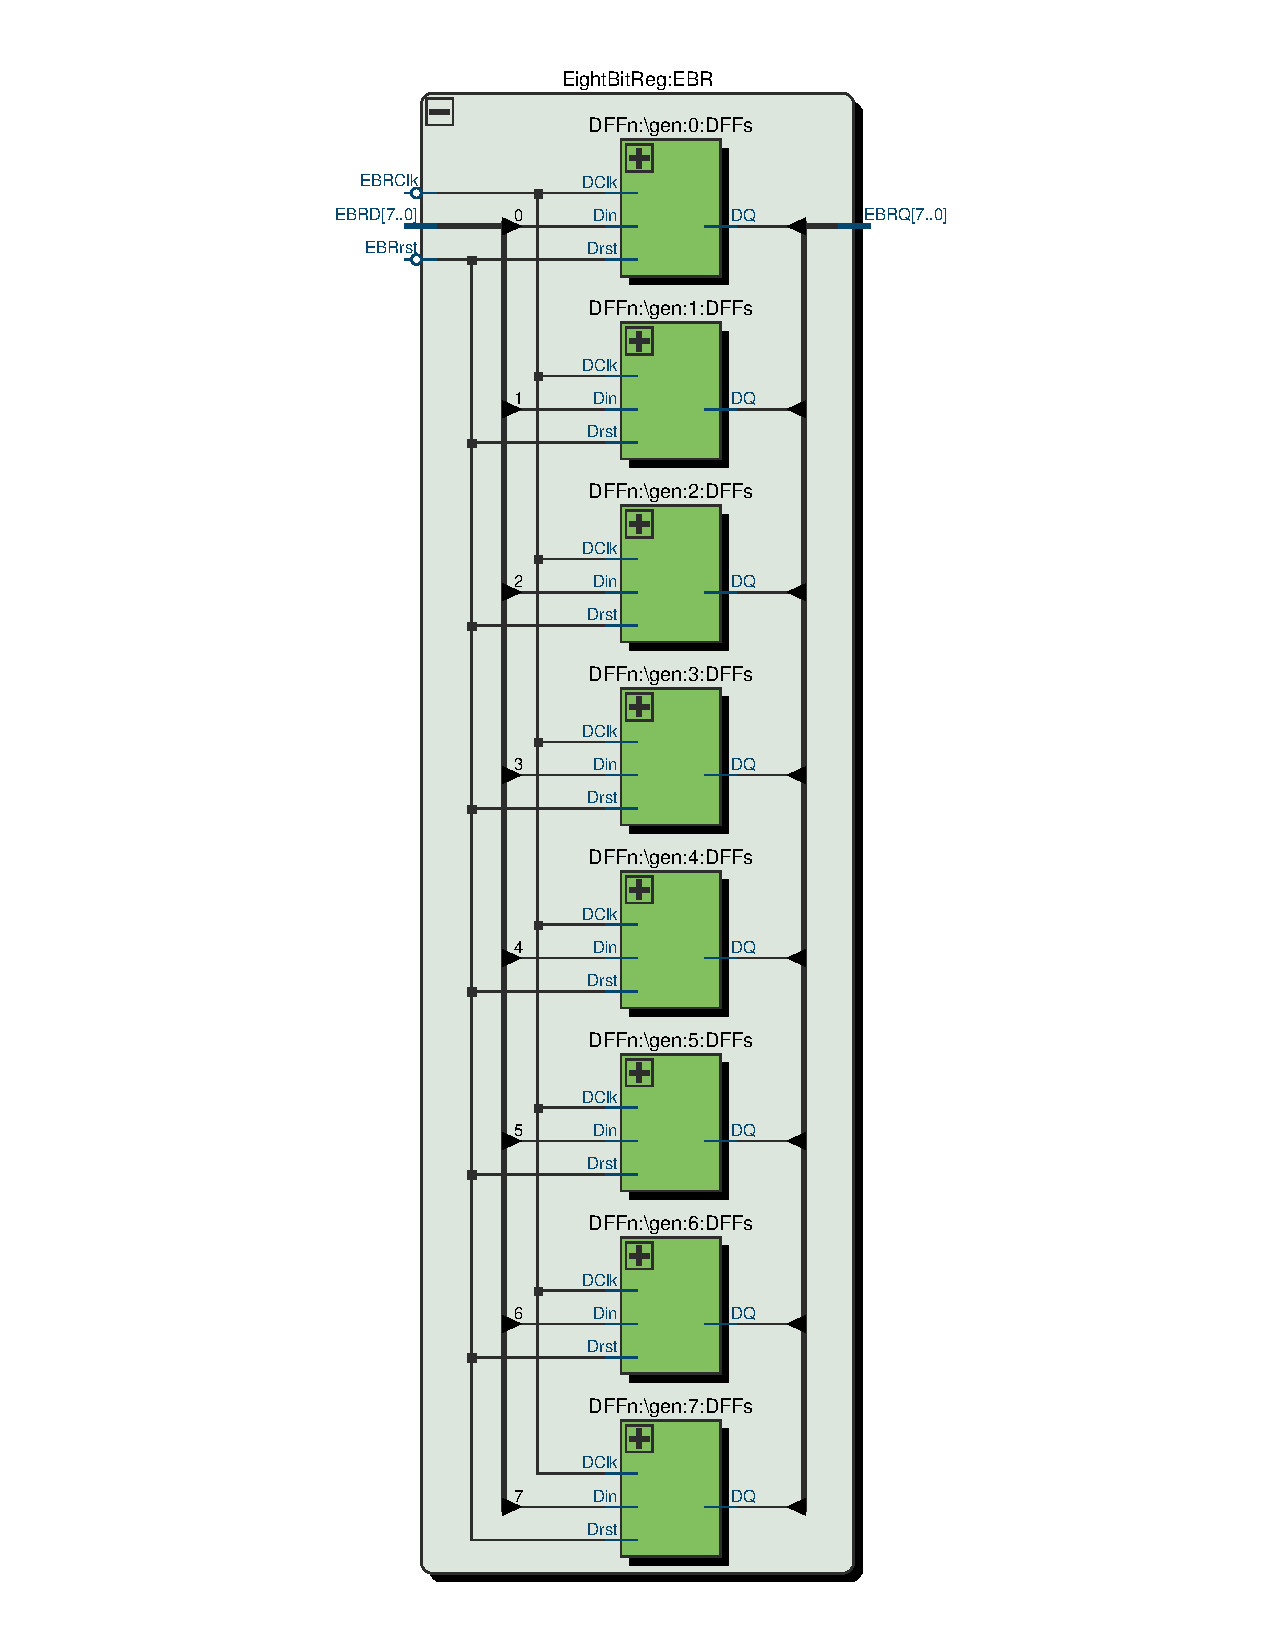
\includegraphics[scale=0.45, clip, trim={2cm 1cm 2cm 1.6cm}]{images/Exc6_EightBitReg_RTL.pdf}}
\end{figure}

\begin{figure}[H]
\centering
\includegraphics[scale=0.55, clip, trim={0cm 3cm 0cm 3.6cm}]{images/Exc6_HEXDisplay_RTL.pdf}
\caption*{HEX display decoder}
\end{figure}

\begin{figure}[H]
\centering
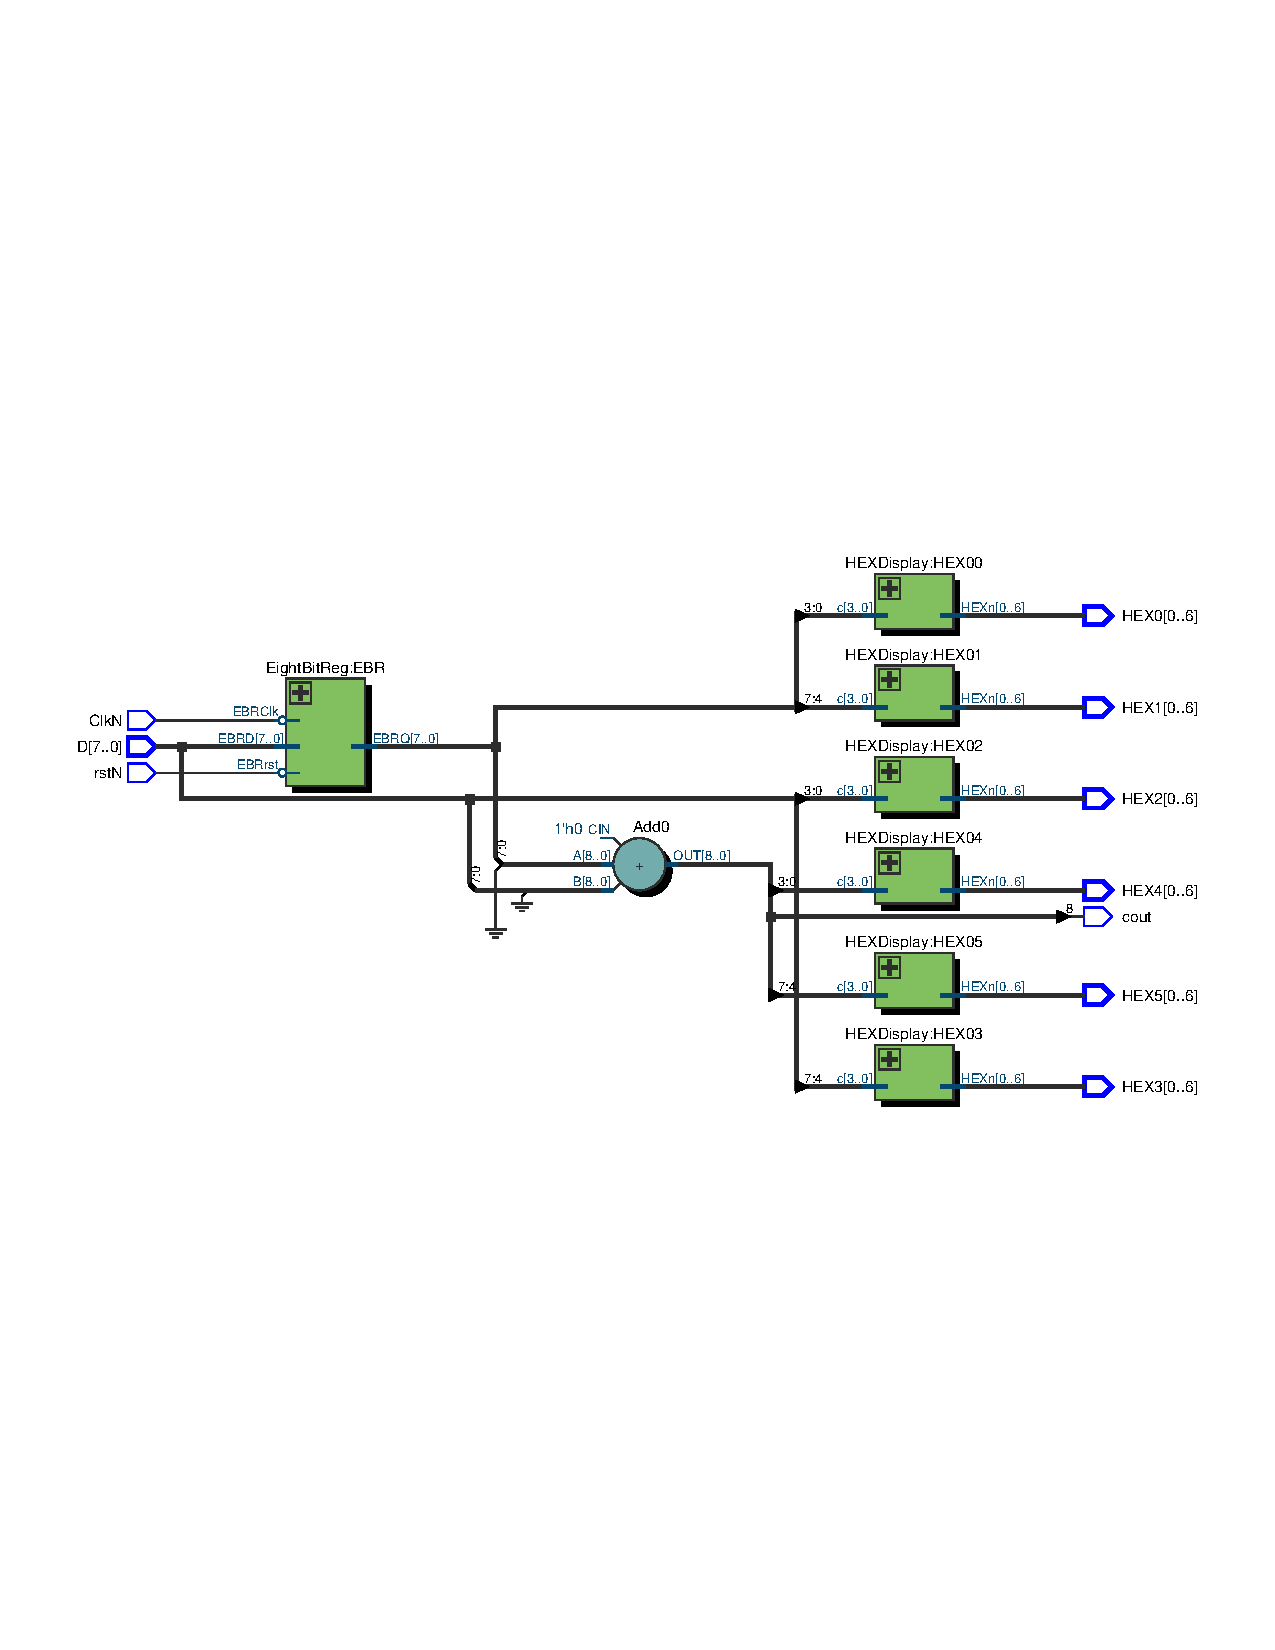
\includegraphics[scale=0.85, clip, trim={0cm 9cm 0cm 9cm}]{images/Exc6_RTL.pdf}
\caption*{Top level}
\end{figure}

\end{document}